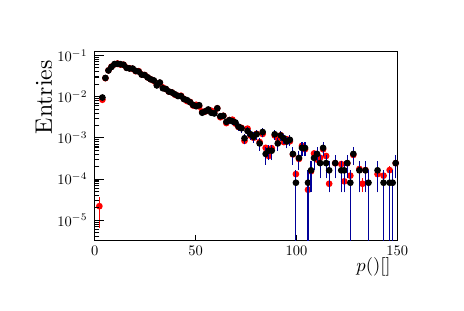
\begin{tikzpicture}
\pgfdeclareplotmark{cross} {
\pgfpathmoveto{\pgfpoint{-0.3\pgfplotmarksize}{\pgfplotmarksize}}
\pgfpathlineto{\pgfpoint{+0.3\pgfplotmarksize}{\pgfplotmarksize}}
\pgfpathlineto{\pgfpoint{+0.3\pgfplotmarksize}{0.3\pgfplotmarksize}}
\pgfpathlineto{\pgfpoint{+1\pgfplotmarksize}{0.3\pgfplotmarksize}}
\pgfpathlineto{\pgfpoint{+1\pgfplotmarksize}{-0.3\pgfplotmarksize}}
\pgfpathlineto{\pgfpoint{+0.3\pgfplotmarksize}{-0.3\pgfplotmarksize}}
\pgfpathlineto{\pgfpoint{+0.3\pgfplotmarksize}{-1.\pgfplotmarksize}}
\pgfpathlineto{\pgfpoint{-0.3\pgfplotmarksize}{-1.\pgfplotmarksize}}
\pgfpathlineto{\pgfpoint{-0.3\pgfplotmarksize}{-0.3\pgfplotmarksize}}
\pgfpathlineto{\pgfpoint{-1.\pgfplotmarksize}{-0.3\pgfplotmarksize}}
\pgfpathlineto{\pgfpoint{-1.\pgfplotmarksize}{0.3\pgfplotmarksize}}
\pgfpathlineto{\pgfpoint{-0.3\pgfplotmarksize}{0.3\pgfplotmarksize}}
\pgfpathclose
\pgfusepathqstroke
}
\pgfdeclareplotmark{cross*} {
\pgfpathmoveto{\pgfpoint{-0.3\pgfplotmarksize}{\pgfplotmarksize}}
\pgfpathlineto{\pgfpoint{+0.3\pgfplotmarksize}{\pgfplotmarksize}}
\pgfpathlineto{\pgfpoint{+0.3\pgfplotmarksize}{0.3\pgfplotmarksize}}
\pgfpathlineto{\pgfpoint{+1\pgfplotmarksize}{0.3\pgfplotmarksize}}
\pgfpathlineto{\pgfpoint{+1\pgfplotmarksize}{-0.3\pgfplotmarksize}}
\pgfpathlineto{\pgfpoint{+0.3\pgfplotmarksize}{-0.3\pgfplotmarksize}}
\pgfpathlineto{\pgfpoint{+0.3\pgfplotmarksize}{-1.\pgfplotmarksize}}
\pgfpathlineto{\pgfpoint{-0.3\pgfplotmarksize}{-1.\pgfplotmarksize}}
\pgfpathlineto{\pgfpoint{-0.3\pgfplotmarksize}{-0.3\pgfplotmarksize}}
\pgfpathlineto{\pgfpoint{-1.\pgfplotmarksize}{-0.3\pgfplotmarksize}}
\pgfpathlineto{\pgfpoint{-1.\pgfplotmarksize}{0.3\pgfplotmarksize}}
\pgfpathlineto{\pgfpoint{-0.3\pgfplotmarksize}{0.3\pgfplotmarksize}}
\pgfpathclose
\pgfusepathqfillstroke
}
\pgfdeclareplotmark{newstar} {
\pgfpathmoveto{\pgfqpoint{0pt}{\pgfplotmarksize}}
\pgfpathlineto{\pgfqpointpolar{44}{0.5\pgfplotmarksize}}
\pgfpathlineto{\pgfqpointpolar{18}{\pgfplotmarksize}}
\pgfpathlineto{\pgfqpointpolar{-20}{0.5\pgfplotmarksize}}
\pgfpathlineto{\pgfqpointpolar{-54}{\pgfplotmarksize}}
\pgfpathlineto{\pgfqpointpolar{-90}{0.5\pgfplotmarksize}}
\pgfpathlineto{\pgfqpointpolar{234}{\pgfplotmarksize}}
\pgfpathlineto{\pgfqpointpolar{198}{0.5\pgfplotmarksize}}
\pgfpathlineto{\pgfqpointpolar{162}{\pgfplotmarksize}}
\pgfpathlineto{\pgfqpointpolar{134}{0.5\pgfplotmarksize}}
\pgfpathclose
\pgfusepathqstroke
}
\pgfdeclareplotmark{newstar*} {
\pgfpathmoveto{\pgfqpoint{0pt}{\pgfplotmarksize}}
\pgfpathlineto{\pgfqpointpolar{44}{0.5\pgfplotmarksize}}
\pgfpathlineto{\pgfqpointpolar{18}{\pgfplotmarksize}}
\pgfpathlineto{\pgfqpointpolar{-20}{0.5\pgfplotmarksize}}
\pgfpathlineto{\pgfqpointpolar{-54}{\pgfplotmarksize}}
\pgfpathlineto{\pgfqpointpolar{-90}{0.5\pgfplotmarksize}}
\pgfpathlineto{\pgfqpointpolar{234}{\pgfplotmarksize}}
\pgfpathlineto{\pgfqpointpolar{198}{0.5\pgfplotmarksize}}
\pgfpathlineto{\pgfqpointpolar{162}{\pgfplotmarksize}}
\pgfpathlineto{\pgfqpointpolar{134}{0.5\pgfplotmarksize}}
\pgfpathclose
\pgfusepathqfillstroke
}
\definecolor{c}{rgb}{1,1,1};
\draw [color=c, fill=c] (5.1,0.0624161) rectangle (9.9,3.05839);
\draw [color=c, fill=c] (5.58,0.362013) rectangle (9.42,2.75879);
\definecolor{c}{rgb}{0,0,0};
\draw [c] (5.58,0.362013) -- (5.58,2.75879) -- (9.42,2.75879) -- (9.42,0.362013) -- (5.58,0.362013);
\definecolor{c}{rgb}{1,0,0};
\draw [c] (5.6376,0.519539) -- (5.6376,0.798603);
\draw [c] (5.6376,0.798603) -- (5.6376,0.920142);
\draw [c] (5.6184,0.798603) -- (5.6376,0.798603);
\draw [c] (5.6376,0.798603) -- (5.6568,0.798603);
\foreach \P in {(5.6376,0.798603)}{\draw[mark options={color=c,fill=c},mark size=2.402402pt,mark=*,mark size=1pt] plot coordinates {\P};}
\draw [c] (5.676,2.142) -- (5.676,2.15036);
\draw [c] (5.676,2.15036) -- (5.676,2.15843);
\draw [c] (5.6568,2.15036) -- (5.676,2.15036);
\draw [c] (5.676,2.15036) -- (5.6952,2.15036);
\foreach \P in {(5.676,2.15036)}{\draw[mark options={color=c,fill=c},mark size=2.402402pt,mark=*,mark size=1pt] plot coordinates {\P};}
\draw [c] (5.7144,2.41958) -- (5.7144,2.42412);
\draw [c] (5.7144,2.42412) -- (5.7144,2.42858);
\draw [c] (5.6952,2.42412) -- (5.7144,2.42412);
\draw [c] (5.7144,2.42412) -- (5.7336,2.42412);
\foreach \P in {(5.7144,2.42412)}{\draw[mark options={color=c,fill=c},mark size=2.402402pt,mark=*,mark size=1pt] plot coordinates {\P};}
\draw [c] (5.7528,2.51937) -- (5.7528,2.52302);
\draw [c] (5.7528,2.52302) -- (5.7528,2.52661);
\draw [c] (5.7336,2.52302) -- (5.7528,2.52302);
\draw [c] (5.7528,2.52302) -- (5.772,2.52302);
\foreach \P in {(5.7528,2.52302)}{\draw[mark options={color=c,fill=c},mark size=2.402402pt,mark=*,mark size=1pt] plot coordinates {\P};}
\draw [c] (5.7912,2.56767) -- (5.7912,2.57095);
\draw [c] (5.7912,2.57095) -- (5.7912,2.57418);
\draw [c] (5.772,2.57095) -- (5.7912,2.57095);
\draw [c] (5.7912,2.57095) -- (5.8104,2.57095);
\foreach \P in {(5.7912,2.57095)}{\draw[mark options={color=c,fill=c},mark size=2.402402pt,mark=*,mark size=1pt] plot coordinates {\P};}
\draw [c] (5.8296,2.59565) -- (5.8296,2.59874);
\draw [c] (5.8296,2.59874) -- (5.8296,2.60178);
\draw [c] (5.8104,2.59874) -- (5.8296,2.59874);
\draw [c] (5.8296,2.59874) -- (5.8488,2.59874);
\foreach \P in {(5.8296,2.59874)}{\draw[mark options={color=c,fill=c},mark size=2.402402pt,mark=*,mark size=1pt] plot coordinates {\P};}
\draw [c] (5.868,2.60759) -- (5.868,2.61059);
\draw [c] (5.868,2.61059) -- (5.868,2.61355);
\draw [c] (5.8488,2.61059) -- (5.868,2.61059);
\draw [c] (5.868,2.61059) -- (5.8872,2.61059);
\foreach \P in {(5.868,2.61059)}{\draw[mark options={color=c,fill=c},mark size=2.402402pt,mark=*,mark size=1pt] plot coordinates {\P};}
\draw [c] (5.9064,2.59294) -- (5.9064,2.59604);
\draw [c] (5.9064,2.59604) -- (5.9064,2.5991);
\draw [c] (5.8872,2.59604) -- (5.9064,2.59604);
\draw [c] (5.9064,2.59604) -- (5.9256,2.59604);
\foreach \P in {(5.9064,2.59604)}{\draw[mark options={color=c,fill=c},mark size=2.402402pt,mark=*,mark size=1pt] plot coordinates {\P};}
\draw [c] (5.9448,2.59167) -- (5.9448,2.59478);
\draw [c] (5.9448,2.59478) -- (5.9448,2.59785);
\draw [c] (5.9256,2.59478) -- (5.9448,2.59478);
\draw [c] (5.9448,2.59478) -- (5.964,2.59478);
\foreach \P in {(5.9448,2.59478)}{\draw[mark options={color=c,fill=c},mark size=2.402402pt,mark=*,mark size=1pt] plot coordinates {\P};}
\draw [c] (5.9832,2.55423) -- (5.9832,2.55761);
\draw [c] (5.9832,2.55761) -- (5.9832,2.56093);
\draw [c] (5.964,2.55761) -- (5.9832,2.55761);
\draw [c] (5.9832,2.55761) -- (6.0024,2.55761);
\foreach \P in {(5.9832,2.55761)}{\draw[mark options={color=c,fill=c},mark size=2.402402pt,mark=*,mark size=1pt] plot coordinates {\P};}
\draw [c] (6.0216,2.5455) -- (6.0216,2.54894);
\draw [c] (6.0216,2.54894) -- (6.0216,2.55233);
\draw [c] (6.0024,2.54894) -- (6.0216,2.54894);
\draw [c] (6.0216,2.54894) -- (6.0408,2.54894);
\foreach \P in {(6.0216,2.54894)}{\draw[mark options={color=c,fill=c},mark size=2.402402pt,mark=*,mark size=1pt] plot coordinates {\P};}
\draw [c] (6.06,2.53915) -- (6.06,2.54264);
\draw [c] (6.06,2.54264) -- (6.06,2.54608);
\draw [c] (6.0408,2.54264) -- (6.06,2.54264);
\draw [c] (6.06,2.54264) -- (6.0792,2.54264);
\foreach \P in {(6.06,2.54264)}{\draw[mark options={color=c,fill=c},mark size=2.402402pt,mark=*,mark size=1pt] plot coordinates {\P};}
\draw [c] (6.0984,2.50929) -- (6.0984,2.51302);
\draw [c] (6.0984,2.51302) -- (6.0984,2.51668);
\draw [c] (6.0792,2.51302) -- (6.0984,2.51302);
\draw [c] (6.0984,2.51302) -- (6.1176,2.51302);
\foreach \P in {(6.0984,2.51302)}{\draw[mark options={color=c,fill=c},mark size=2.402402pt,mark=*,mark size=1pt] plot coordinates {\P};}
\draw [c] (6.1368,2.50959) -- (6.1368,2.51332);
\draw [c] (6.1368,2.51332) -- (6.1368,2.51698);
\draw [c] (6.1176,2.51332) -- (6.1368,2.51332);
\draw [c] (6.1368,2.51332) -- (6.156,2.51332);
\foreach \P in {(6.1368,2.51332)}{\draw[mark options={color=c,fill=c},mark size=2.402402pt,mark=*,mark size=1pt] plot coordinates {\P};}
\draw [c] (6.1752,2.4663) -- (6.1752,2.4704);
\draw [c] (6.1752,2.4704) -- (6.1752,2.47442);
\draw [c] (6.156,2.4704) -- (6.1752,2.4704);
\draw [c] (6.1752,2.4704) -- (6.1944,2.4704);
\foreach \P in {(6.1752,2.4704)}{\draw[mark options={color=c,fill=c},mark size=2.402402pt,mark=*,mark size=1pt] plot coordinates {\P};}
\draw [c] (6.2136,2.45969) -- (6.2136,2.46385);
\draw [c] (6.2136,2.46385) -- (6.2136,2.46793);
\draw [c] (6.1944,2.46385) -- (6.2136,2.46385);
\draw [c] (6.2136,2.46385) -- (6.2328,2.46385);
\foreach \P in {(6.2136,2.46385)}{\draw[mark options={color=c,fill=c},mark size=2.402402pt,mark=*,mark size=1pt] plot coordinates {\P};}
\draw [c] (6.252,2.42831) -- (6.252,2.43276);
\draw [c] (6.252,2.43276) -- (6.252,2.43713);
\draw [c] (6.2328,2.43276) -- (6.252,2.43276);
\draw [c] (6.252,2.43276) -- (6.2712,2.43276);
\foreach \P in {(6.252,2.43276)}{\draw[mark options={color=c,fill=c},mark size=2.402402pt,mark=*,mark size=1pt] plot coordinates {\P};}
\draw [c] (6.2904,2.40483) -- (6.2904,2.40952);
\draw [c] (6.2904,2.40952) -- (6.2904,2.41412);
\draw [c] (6.2712,2.40952) -- (6.2904,2.40952);
\draw [c] (6.2904,2.40952) -- (6.3096,2.40952);
\foreach \P in {(6.2904,2.40952)}{\draw[mark options={color=c,fill=c},mark size=2.402402pt,mark=*,mark size=1pt] plot coordinates {\P};}
\draw [c] (6.3288,2.38575) -- (6.3288,2.39064);
\draw [c] (6.3288,2.39064) -- (6.3288,2.39543);
\draw [c] (6.3096,2.39064) -- (6.3288,2.39064);
\draw [c] (6.3288,2.39064) -- (6.348,2.39064);
\foreach \P in {(6.3288,2.39064)}{\draw[mark options={color=c,fill=c},mark size=2.402402pt,mark=*,mark size=1pt] plot coordinates {\P};}
\draw [c] (6.3672,2.33524) -- (6.3672,2.3407);
\draw [c] (6.3672,2.3407) -- (6.3672,2.34604);
\draw [c] (6.348,2.3407) -- (6.3672,2.3407);
\draw [c] (6.3672,2.3407) -- (6.3864,2.3407);
\foreach \P in {(6.3672,2.3407)}{\draw[mark options={color=c,fill=c},mark size=2.402402pt,mark=*,mark size=1pt] plot coordinates {\P};}
\draw [c] (6.4056,2.35868) -- (6.4056,2.36388);
\draw [c] (6.4056,2.36388) -- (6.4056,2.36895);
\draw [c] (6.3864,2.36388) -- (6.4056,2.36388);
\draw [c] (6.4056,2.36388) -- (6.4248,2.36388);
\foreach \P in {(6.4056,2.36388)}{\draw[mark options={color=c,fill=c},mark size=2.402402pt,mark=*,mark size=1pt] plot coordinates {\P};}
\draw [c] (6.444,2.30019) -- (6.444,2.3061);
\draw [c] (6.444,2.3061) -- (6.444,2.31185);
\draw [c] (6.4248,2.3061) -- (6.444,2.3061);
\draw [c] (6.444,2.3061) -- (6.4632,2.3061);
\foreach \P in {(6.444,2.3061)}{\draw[mark options={color=c,fill=c},mark size=2.402402pt,mark=*,mark size=1pt] plot coordinates {\P};}
\draw [c] (6.4824,2.27844) -- (6.4824,2.28463);
\draw [c] (6.4824,2.28463) -- (6.4824,2.29066);
\draw [c] (6.4632,2.28463) -- (6.4824,2.28463);
\draw [c] (6.4824,2.28463) -- (6.5016,2.28463);
\foreach \P in {(6.4824,2.28463)}{\draw[mark options={color=c,fill=c},mark size=2.402402pt,mark=*,mark size=1pt] plot coordinates {\P};}
\draw [c] (6.5208,2.24649) -- (6.5208,2.25313);
\draw [c] (6.5208,2.25313) -- (6.5208,2.25959);
\draw [c] (6.5016,2.25313) -- (6.5208,2.25313);
\draw [c] (6.5208,2.25313) -- (6.54,2.25313);
\foreach \P in {(6.5208,2.25313)}{\draw[mark options={color=c,fill=c},mark size=2.402402pt,mark=*,mark size=1pt] plot coordinates {\P};}
\draw [c] (6.5592,2.2361) -- (6.5592,2.2429);
\draw [c] (6.5592,2.2429) -- (6.5592,2.2495);
\draw [c] (6.54,2.2429) -- (6.5592,2.2429);
\draw [c] (6.5592,2.2429) -- (6.5784,2.2429);
\foreach \P in {(6.5592,2.2429)}{\draw[mark options={color=c,fill=c},mark size=2.402402pt,mark=*,mark size=1pt] plot coordinates {\P};}
\draw [c] (6.5976,2.20753) -- (6.5976,2.21477);
\draw [c] (6.5976,2.21477) -- (6.5976,2.22179);
\draw [c] (6.5784,2.21477) -- (6.5976,2.21477);
\draw [c] (6.5976,2.21477) -- (6.6168,2.21477);
\foreach \P in {(6.5976,2.21477)}{\draw[mark options={color=c,fill=c},mark size=2.402402pt,mark=*,mark size=1pt] plot coordinates {\P};}
\draw [c] (6.636,2.193) -- (6.636,2.20048);
\draw [c] (6.636,2.20048) -- (6.636,2.20771);
\draw [c] (6.6168,2.20048) -- (6.636,2.20048);
\draw [c] (6.636,2.20048) -- (6.6552,2.20048);
\foreach \P in {(6.636,2.20048)}{\draw[mark options={color=c,fill=c},mark size=2.402402pt,mark=*,mark size=1pt] plot coordinates {\P};}
\draw [c] (6.6744,2.19348) -- (6.6744,2.20095);
\draw [c] (6.6744,2.20095) -- (6.6744,2.20818);
\draw [c] (6.6552,2.20095) -- (6.6744,2.20095);
\draw [c] (6.6744,2.20095) -- (6.6936,2.20095);
\foreach \P in {(6.6744,2.20095)}{\draw[mark options={color=c,fill=c},mark size=2.402402pt,mark=*,mark size=1pt] plot coordinates {\P};}
\draw [c] (6.7128,2.1506) -- (6.7128,2.1588);
\draw [c] (6.7128,2.1588) -- (6.7128,2.16672);
\draw [c] (6.6936,2.1588) -- (6.7128,2.1588);
\draw [c] (6.7128,2.1588) -- (6.732,2.1588);
\foreach \P in {(6.7128,2.1588)}{\draw[mark options={color=c,fill=c},mark size=2.402402pt,mark=*,mark size=1pt] plot coordinates {\P};}
\draw [c] (6.7512,2.12441) -- (6.7512,2.13311);
\draw [c] (6.7512,2.13311) -- (6.7512,2.14148);
\draw [c] (6.732,2.13311) -- (6.7512,2.13311);
\draw [c] (6.7512,2.13311) -- (6.7704,2.13311);
\foreach \P in {(6.7512,2.13311)}{\draw[mark options={color=c,fill=c},mark size=2.402402pt,mark=*,mark size=1pt] plot coordinates {\P};}
\draw [c] (6.7896,2.11373) -- (6.7896,2.12263);
\draw [c] (6.7896,2.12263) -- (6.7896,2.13119);
\draw [c] (6.7704,2.12263) -- (6.7896,2.12263);
\draw [c] (6.7896,2.12263) -- (6.8088,2.12263);
\foreach \P in {(6.7896,2.12263)}{\draw[mark options={color=c,fill=c},mark size=2.402402pt,mark=*,mark size=1pt] plot coordinates {\P};}
\draw [c] (6.828,2.06728) -- (6.828,2.07713);
\draw [c] (6.828,2.07713) -- (6.828,2.08658);
\draw [c] (6.8088,2.07713) -- (6.828,2.07713);
\draw [c] (6.828,2.07713) -- (6.8472,2.07713);
\foreach \P in {(6.828,2.07713)}{\draw[mark options={color=c,fill=c},mark size=2.402402pt,mark=*,mark size=1pt] plot coordinates {\P};}
\draw [c] (6.8664,2.07671) -- (6.8664,2.08636);
\draw [c] (6.8664,2.08636) -- (6.8664,2.09562);
\draw [c] (6.8472,2.08636) -- (6.8664,2.08636);
\draw [c] (6.8664,2.08636) -- (6.8856,2.08636);
\foreach \P in {(6.8664,2.08636)}{\draw[mark options={color=c,fill=c},mark size=2.402402pt,mark=*,mark size=1pt] plot coordinates {\P};}
\draw [c] (6.9048,2.05436) -- (6.9048,2.0645);
\draw [c] (6.9048,2.0645) -- (6.9048,2.07421);
\draw [c] (6.8856,2.0645) -- (6.9048,2.0645);
\draw [c] (6.9048,2.0645) -- (6.924,2.0645);
\foreach \P in {(6.9048,2.0645)}{\draw[mark options={color=c,fill=c},mark size=2.402402pt,mark=*,mark size=1pt] plot coordinates {\P};}
\draw [c] (6.9432,1.98633) -- (6.9432,1.99811);
\draw [c] (6.9432,1.99811) -- (6.9432,2.00931);
\draw [c] (6.924,1.99811) -- (6.9432,1.99811);
\draw [c] (6.9432,1.99811) -- (6.9624,1.99811);
\foreach \P in {(6.9432,1.99811)}{\draw[mark options={color=c,fill=c},mark size=2.402402pt,mark=*,mark size=1pt] plot coordinates {\P};}
\draw [c] (6.9816,1.9887) -- (6.9816,2.00042);
\draw [c] (6.9816,2.00042) -- (6.9816,2.01156);
\draw [c] (6.9624,2.00042) -- (6.9816,2.00042);
\draw [c] (6.9816,2.00042) -- (7.0008,2.00042);
\foreach \P in {(6.9816,2.00042)}{\draw[mark options={color=c,fill=c},mark size=2.402402pt,mark=*,mark size=1pt] plot coordinates {\P};}
\draw [c] (7.02,2.00242) -- (7.02,2.01379);
\draw [c] (7.02,2.01379) -- (7.02,2.02462);
\draw [c] (7.0008,2.01379) -- (7.02,2.01379);
\draw [c] (7.02,2.01379) -- (7.0392,2.01379);
\foreach \P in {(7.02,2.01379)}{\draw[mark options={color=c,fill=c},mark size=2.402402pt,mark=*,mark size=1pt] plot coordinates {\P};}
\draw [c] (7.0584,1.99907) -- (7.0584,2.01052);
\draw [c] (7.0584,2.01052) -- (7.0584,2.02143);
\draw [c] (7.0392,2.01052) -- (7.0584,2.01052);
\draw [c] (7.0584,2.01052) -- (7.0776,2.01052);
\foreach \P in {(7.0584,2.01052)}{\draw[mark options={color=c,fill=c},mark size=2.402402pt,mark=*,mark size=1pt] plot coordinates {\P};}
\draw [c] (7.0968,1.97411) -- (7.0968,1.98621);
\draw [c] (7.0968,1.98621) -- (7.0968,1.9977);
\draw [c] (7.0776,1.98621) -- (7.0968,1.98621);
\draw [c] (7.0968,1.98621) -- (7.116,1.98621);
\foreach \P in {(7.0968,1.98621)}{\draw[mark options={color=c,fill=c},mark size=2.402402pt,mark=*,mark size=1pt] plot coordinates {\P};}
\draw [c] (7.1352,2.03059) -- (7.1352,2.04128);
\draw [c] (7.1352,2.04128) -- (7.1352,2.05149);
\draw [c] (7.116,2.04128) -- (7.1352,2.04128);
\draw [c] (7.1352,2.04128) -- (7.1544,2.04128);
\foreach \P in {(7.1352,2.04128)}{\draw[mark options={color=c,fill=c},mark size=2.402402pt,mark=*,mark size=1pt] plot coordinates {\P};}
\draw [c] (7.1736,1.91425) -- (7.1736,1.92805);
\draw [c] (7.1736,1.92805) -- (7.1736,1.94106);
\draw [c] (7.1544,1.92805) -- (7.1736,1.92805);
\draw [c] (7.1736,1.92805) -- (7.1928,1.92805);
\foreach \P in {(7.1736,1.92805)}{\draw[mark options={color=c,fill=c},mark size=2.402402pt,mark=*,mark size=1pt] plot coordinates {\P};}
\draw [c] (7.212,1.93299) -- (7.212,1.94624);
\draw [c] (7.212,1.94624) -- (7.212,1.95875);
\draw [c] (7.1928,1.94624) -- (7.212,1.94624);
\draw [c] (7.212,1.94624) -- (7.2312,1.94624);
\foreach \P in {(7.212,1.94624)}{\draw[mark options={color=c,fill=c},mark size=2.402402pt,mark=*,mark size=1pt] plot coordinates {\P};}
\draw [c] (7.2504,1.83776) -- (7.2504,1.85409);
\draw [c] (7.2504,1.85409) -- (7.2504,1.86933);
\draw [c] (7.2312,1.85409) -- (7.2504,1.85409);
\draw [c] (7.2504,1.85409) -- (7.2696,1.85409);
\foreach \P in {(7.2504,1.85409)}{\draw[mark options={color=c,fill=c},mark size=2.402402pt,mark=*,mark size=1pt] plot coordinates {\P};}
\draw [c] (7.2888,1.87725) -- (7.2888,1.89222);
\draw [c] (7.2888,1.89222) -- (7.2888,1.90627);
\draw [c] (7.2696,1.89222) -- (7.2888,1.89222);
\draw [c] (7.2888,1.89222) -- (7.308,1.89222);
\foreach \P in {(7.2888,1.89222)}{\draw[mark options={color=c,fill=c},mark size=2.402402pt,mark=*,mark size=1pt] plot coordinates {\P};}
\draw [c] (7.3272,1.88198) -- (7.3272,1.8968);
\draw [c] (7.3272,1.8968) -- (7.3272,1.91071);
\draw [c] (7.308,1.8968) -- (7.3272,1.8968);
\draw [c] (7.3272,1.8968) -- (7.3464,1.8968);
\foreach \P in {(7.3272,1.8968)}{\draw[mark options={color=c,fill=c},mark size=2.402402pt,mark=*,mark size=1pt] plot coordinates {\P};}
\draw [c] (7.3656,1.83086) -- (7.3656,1.84744);
\draw [c] (7.3656,1.84744) -- (7.3656,1.86289);
\draw [c] (7.3464,1.84744) -- (7.3656,1.84744);
\draw [c] (7.3656,1.84744) -- (7.3848,1.84744);
\foreach \P in {(7.3656,1.84744)}{\draw[mark options={color=c,fill=c},mark size=2.402402pt,mark=*,mark size=1pt] plot coordinates {\P};}
\draw [c] (7.404,1.78589) -- (7.404,1.8042);
\draw [c] (7.404,1.8042) -- (7.404,1.82114);
\draw [c] (7.3848,1.8042) -- (7.404,1.8042);
\draw [c] (7.404,1.8042) -- (7.4232,1.8042);
\foreach \P in {(7.404,1.8042)}{\draw[mark options={color=c,fill=c},mark size=2.402402pt,mark=*,mark size=1pt] plot coordinates {\P};}
\draw [c] (7.4424,1.77426) -- (7.4424,1.79304);
\draw [c] (7.4424,1.79304) -- (7.4424,1.81039);
\draw [c] (7.4232,1.79304) -- (7.4424,1.79304);
\draw [c] (7.4424,1.79304) -- (7.4616,1.79304);
\foreach \P in {(7.4424,1.79304)}{\draw[mark options={color=c,fill=c},mark size=2.402402pt,mark=*,mark size=1pt] plot coordinates {\P};}
\draw [c] (7.4808,1.60076) -- (7.4808,1.62826);
\draw [c] (7.4808,1.62826) -- (7.4808,1.65278);
\draw [c] (7.4616,1.62826) -- (7.4808,1.62826);
\draw [c] (7.4808,1.62826) -- (7.5,1.62826);
\foreach \P in {(7.4808,1.62826)}{\draw[mark options={color=c,fill=c},mark size=2.402402pt,mark=*,mark size=1pt] plot coordinates {\P};}
\draw [c] (7.5192,1.76359) -- (7.5192,1.78281);
\draw [c] (7.5192,1.78281) -- (7.5192,1.80053);
\draw [c] (7.5,1.78281) -- (7.5192,1.78281);
\draw [c] (7.5192,1.78281) -- (7.5384,1.78281);
\foreach \P in {(7.5192,1.78281)}{\draw[mark options={color=c,fill=c},mark size=2.402402pt,mark=*,mark size=1pt] plot coordinates {\P};}
\draw [c] (7.5576,1.6708) -- (7.5576,1.69437);
\draw [c] (7.5576,1.69437) -- (7.5576,1.71573);
\draw [c] (7.5384,1.69437) -- (7.5576,1.69437);
\draw [c] (7.5576,1.69437) -- (7.5768,1.69437);
\foreach \P in {(7.5576,1.69437)}{\draw[mark options={color=c,fill=c},mark size=2.402402pt,mark=*,mark size=1pt] plot coordinates {\P};}
\draw [c] (7.596,1.64105) -- (7.596,1.66622);
\draw [c] (7.596,1.66622) -- (7.596,1.68888);
\draw [c] (7.5768,1.66622) -- (7.596,1.66622);
\draw [c] (7.596,1.66622) -- (7.6152,1.66622);
\foreach \P in {(7.596,1.66622)}{\draw[mark options={color=c,fill=c},mark size=2.402402pt,mark=*,mark size=1pt] plot coordinates {\P};}
\draw [c] (7.6344,1.69508) -- (7.6344,1.71743);
\draw [c] (7.6344,1.71743) -- (7.6344,1.73778);
\draw [c] (7.6152,1.71743) -- (7.6344,1.71743);
\draw [c] (7.6344,1.71743) -- (7.6536,1.71743);
\foreach \P in {(7.6344,1.71743)}{\draw[mark options={color=c,fill=c},mark size=2.402402pt,mark=*,mark size=1pt] plot coordinates {\P};}
\draw [c] (7.6728,1.5845) -- (7.6728,1.613);
\draw [c] (7.6728,1.613) -- (7.6728,1.63832);
\draw [c] (7.6536,1.613) -- (7.6728,1.613);
\draw [c] (7.6728,1.613) -- (7.692,1.613);
\foreach \P in {(7.6728,1.613)}{\draw[mark options={color=c,fill=c},mark size=2.402402pt,mark=*,mark size=1pt] plot coordinates {\P};}
\draw [c] (7.7112,1.69298) -- (7.7112,1.71543);
\draw [c] (7.7112,1.71543) -- (7.7112,1.73586);
\draw [c] (7.692,1.71543) -- (7.7112,1.71543);
\draw [c] (7.7112,1.71543) -- (7.7304,1.71543);
\foreach \P in {(7.7112,1.71543)}{\draw[mark options={color=c,fill=c},mark size=2.402402pt,mark=*,mark size=1pt] plot coordinates {\P};}
\draw [c] (7.7496,1.50512) -- (7.7496,1.53904);
\draw [c] (7.7496,1.53904) -- (7.7496,1.56855);
\draw [c] (7.7304,1.53904) -- (7.7496,1.53904);
\draw [c] (7.7496,1.53904) -- (7.7688,1.53904);
\foreach \P in {(7.7496,1.53904)}{\draw[mark options={color=c,fill=c},mark size=2.402402pt,mark=*,mark size=1pt] plot coordinates {\P};}
\draw [c] (7.788,1.39223) -- (7.788,1.4357);
\draw [c] (7.788,1.4357) -- (7.788,1.47217);
\draw [c] (7.7688,1.4357) -- (7.788,1.4357);
\draw [c] (7.788,1.4357) -- (7.8072,1.4357);
\foreach \P in {(7.788,1.4357)}{\draw[mark options={color=c,fill=c},mark size=2.402402pt,mark=*,mark size=1pt] plot coordinates {\P};}
\draw [c] (7.8264,1.50034) -- (7.8264,1.53463);
\draw [c] (7.8264,1.53463) -- (7.8264,1.56441);
\draw [c] (7.8072,1.53463) -- (7.8264,1.53463);
\draw [c] (7.8264,1.53463) -- (7.8456,1.53463);
\foreach \P in {(7.8264,1.53463)}{\draw[mark options={color=c,fill=c},mark size=2.402402pt,mark=*,mark size=1pt] plot coordinates {\P};}
\draw [c] (7.8648,1.67311) -- (7.8648,1.69657);
\draw [c] (7.8648,1.69657) -- (7.8648,1.71783);
\draw [c] (7.8456,1.69657) -- (7.8648,1.69657);
\draw [c] (7.8648,1.69657) -- (7.884,1.69657);
\foreach \P in {(7.8648,1.69657)}{\draw[mark options={color=c,fill=c},mark size=2.402402pt,mark=*,mark size=1pt] plot coordinates {\P};}
\draw [c] (7.9032,1.63839) -- (7.9032,1.66371);
\draw [c] (7.9032,1.66371) -- (7.9032,1.68648);
\draw [c] (7.884,1.66371) -- (7.9032,1.66371);
\draw [c] (7.9032,1.66371) -- (7.9224,1.66371);
\foreach \P in {(7.9032,1.66371)}{\draw[mark options={color=c,fill=c},mark size=2.402402pt,mark=*,mark size=1pt] plot coordinates {\P};}
\draw [c] (7.9416,1.6754) -- (7.9416,1.69874);
\draw [c] (7.9416,1.69874) -- (7.9416,1.7199);
\draw [c] (7.9224,1.69874) -- (7.9416,1.69874);
\draw [c] (7.9416,1.69874) -- (7.9608,1.69874);
\foreach \P in {(7.9416,1.69874)}{\draw[mark options={color=c,fill=c},mark size=2.402402pt,mark=*,mark size=1pt] plot coordinates {\P};}
\draw [c] (7.98,1.5845) -- (7.98,1.613);
\draw [c] (7.98,1.613) -- (7.98,1.63832);
\draw [c] (7.9608,1.613) -- (7.98,1.613);
\draw [c] (7.98,1.613) -- (7.9992,1.613);
\foreach \P in {(7.98,1.613)}{\draw[mark options={color=c,fill=c},mark size=2.402402pt,mark=*,mark size=1pt] plot coordinates {\P};}
\draw [c] (8.0184,1.62177) -- (8.0184,1.64803);
\draw [c] (8.0184,1.64803) -- (8.0184,1.67156);
\draw [c] (7.9992,1.64803) -- (8.0184,1.64803);
\draw [c] (8.0184,1.64803) -- (8.0376,1.64803);
\foreach \P in {(8.0184,1.64803)}{\draw[mark options={color=c,fill=c},mark size=2.402402pt,mark=*,mark size=1pt] plot coordinates {\P};}
\draw [c] (8.0568,1.59439) -- (8.0568,1.62227);
\draw [c] (8.0568,1.62227) -- (8.0568,1.64711);
\draw [c] (8.0376,1.62227) -- (8.0568,1.62227);
\draw [c] (8.0568,1.62227) -- (8.076,1.62227);
\foreach \P in {(8.0568,1.62227)}{\draw[mark options={color=c,fill=c},mark size=2.402402pt,mark=*,mark size=1pt] plot coordinates {\P};}
\draw [c] (8.0952,1.41404) -- (8.0952,1.45547);
\draw [c] (8.0952,1.45547) -- (8.0952,1.4905);
\draw [c] (8.076,1.45547) -- (8.0952,1.45547);
\draw [c] (8.0952,1.45547) -- (8.1144,1.45547);
\foreach \P in {(8.0952,1.45547)}{\draw[mark options={color=c,fill=c},mark size=2.402402pt,mark=*,mark size=1pt] plot coordinates {\P};}
\draw [c] (8.1336,1.12839) -- (8.1336,1.2058);
\draw [c] (8.1336,1.2058) -- (8.1336,1.26344);
\draw [c] (8.1144,1.2058) -- (8.1336,1.2058);
\draw [c] (8.1336,1.2058) -- (8.1528,1.2058);
\foreach \P in {(8.1336,1.2058)}{\draw[mark options={color=c,fill=c},mark size=2.402402pt,mark=*,mark size=1pt] plot coordinates {\P};}
\draw [c] (8.172,1.35075) -- (8.172,1.39836);
\draw [c] (8.172,1.39836) -- (8.172,1.4377);
\draw [c] (8.1528,1.39836) -- (8.172,1.39836);
\draw [c] (8.172,1.39836) -- (8.1912,1.39836);
\foreach \P in {(8.172,1.39836)}{\draw[mark options={color=c,fill=c},mark size=2.402402pt,mark=*,mark size=1pt] plot coordinates {\P};}
\draw [c] (8.2104,1.53187) -- (8.2104,1.56386);
\draw [c] (8.2104,1.56386) -- (8.2104,1.5919);
\draw [c] (8.1912,1.56386) -- (8.2104,1.56386);
\draw [c] (8.2104,1.56386) -- (8.2296,1.56386);
\foreach \P in {(8.2104,1.56386)}{\draw[mark options={color=c,fill=c},mark size=2.402402pt,mark=*,mark size=1pt] plot coordinates {\P};}
\draw [c] (8.2488,1.48543) -- (8.2488,1.52085);
\draw [c] (8.2488,1.52085) -- (8.2488,1.55149);
\draw [c] (8.2296,1.52085) -- (8.2488,1.52085);
\draw [c] (8.2488,1.52085) -- (8.268,1.52085);
\foreach \P in {(8.2488,1.52085)}{\draw[mark options={color=c,fill=c},mark size=2.402402pt,mark=*,mark size=1pt] plot coordinates {\P};}
\draw [c] (8.2872,0.872124) -- (8.2872,1.00684);
\draw [c] (8.2872,1.00684) -- (8.2872,1.09085);
\draw [c] (8.268,1.00684) -- (8.2872,1.00684);
\draw [c] (8.2872,1.00684) -- (8.3064,1.00684);
\foreach \P in {(8.2872,1.00684)}{\draw[mark options={color=c,fill=c},mark size=2.402402pt,mark=*,mark size=1pt] plot coordinates {\P};}
\draw [c] (8.3256,1.17016) -- (8.3256,1.24083);
\draw [c] (8.3256,1.24083) -- (8.3256,1.29466);
\draw [c] (8.3064,1.24083) -- (8.3256,1.24083);
\draw [c] (8.3256,1.24083) -- (8.3448,1.24083);
\foreach \P in {(8.3256,1.24083)}{\draw[mark options={color=c,fill=c},mark size=2.402402pt,mark=*,mark size=1pt] plot coordinates {\P};}
\draw [c] (8.364,1.42753) -- (8.364,1.46776);
\draw [c] (8.364,1.46776) -- (8.364,1.50192);
\draw [c] (8.3448,1.46776) -- (8.364,1.46776);
\draw [c] (8.364,1.46776) -- (8.3832,1.46776);
\foreach \P in {(8.364,1.46776)}{\draw[mark options={color=c,fill=c},mark size=2.402402pt,mark=*,mark size=1pt] plot coordinates {\P};}
\draw [c] (8.4024,1.34152) -- (8.4024,1.39009);
\draw [c] (8.4024,1.39009) -- (8.4024,1.43009);
\draw [c] (8.3832,1.39009) -- (8.4024,1.39009);
\draw [c] (8.4024,1.39009) -- (8.4216,1.39009);
\foreach \P in {(8.4024,1.39009)}{\draw[mark options={color=c,fill=c},mark size=2.402402pt,mark=*,mark size=1pt] plot coordinates {\P};}
\draw [c] (8.4408,1.36822) -- (8.4408,1.41404);
\draw [c] (8.4408,1.41404) -- (8.4408,1.45215);
\draw [c] (8.4216,1.41404) -- (8.4408,1.41404);
\draw [c] (8.4408,1.41404) -- (8.46,1.41404);
\foreach \P in {(8.4408,1.41404)}{\draw[mark options={color=c,fill=c},mark size=2.402402pt,mark=*,mark size=1pt] plot coordinates {\P};}
\draw [c] (8.4792,1.48543) -- (8.4792,1.52085);
\draw [c] (8.4792,1.52085) -- (8.4792,1.55149);
\draw [c] (8.46,1.52085) -- (8.4792,1.52085);
\draw [c] (8.4792,1.52085) -- (8.4984,1.52085);
\foreach \P in {(8.4792,1.52085)}{\draw[mark options={color=c,fill=c},mark size=2.402402pt,mark=*,mark size=1pt] plot coordinates {\P};}
\draw [c] (8.5176,1.39223) -- (8.5176,1.4357);
\draw [c] (8.5176,1.4357) -- (8.5176,1.47217);
\draw [c] (8.4984,1.4357) -- (8.5176,1.4357);
\draw [c] (8.5176,1.4357) -- (8.5368,1.4357);
\foreach \P in {(8.5176,1.4357)}{\draw[mark options={color=c,fill=c},mark size=2.402402pt,mark=*,mark size=1pt] plot coordinates {\P};}
\draw [c] (8.556,0.975413) -- (8.556,1.08331);
\draw [c] (8.556,1.08331) -- (8.556,1.15617);
\draw [c] (8.5368,1.08331) -- (8.556,1.08331);
\draw [c] (8.556,1.08331) -- (8.5752,1.08331);
\foreach \P in {(8.556,1.08331)}{\draw[mark options={color=c,fill=c},mark size=2.402402pt,mark=*,mark size=1pt] plot coordinates {\P};}
\draw [c] (8.6328,1.28906) -- (8.6328,1.34355);
\draw [c] (8.6328,1.34355) -- (8.6328,1.38747);
\draw [c] (8.6136,1.34355) -- (8.6328,1.34355);
\draw [c] (8.6328,1.34355) -- (8.652,1.34355);
\foreach \P in {(8.6328,1.34355)}{\draw[mark options={color=c,fill=c},mark size=2.402402pt,mark=*,mark size=1pt] plot coordinates {\P};}
\draw [c] (8.7096,1.27703) -- (8.7096,1.33298);
\draw [c] (8.7096,1.33298) -- (8.7096,1.37784);
\draw [c] (8.6904,1.33298) -- (8.7096,1.33298);
\draw [c] (8.7096,1.33298) -- (8.7288,1.33298);
\foreach \P in {(8.7096,1.33298)}{\draw[mark options={color=c,fill=c},mark size=2.402402pt,mark=*,mark size=1pt] plot coordinates {\P};}
\draw [c] (8.748,1.01451) -- (8.748,1.11365);
\draw [c] (8.748,1.11365) -- (8.748,1.18245);
\draw [c] (8.7288,1.11365) -- (8.748,1.11365);
\draw [c] (8.748,1.11365) -- (8.7672,1.11365);
\foreach \P in {(8.748,1.11365)}{\draw[mark options={color=c,fill=c},mark size=2.402402pt,mark=*,mark size=1pt] plot coordinates {\P};}
\draw [c] (8.7864,1.28906) -- (8.7864,1.34355);
\draw [c] (8.7864,1.34355) -- (8.7864,1.38747);
\draw [c] (8.7672,1.34355) -- (8.7864,1.34355);
\draw [c] (8.7864,1.34355) -- (8.8056,1.34355);
\foreach \P in {(8.7864,1.34355)}{\draw[mark options={color=c,fill=c},mark size=2.402402pt,mark=*,mark size=1pt] plot coordinates {\P};}
\draw [c] (8.8248,1.10448) -- (8.8248,1.18603);
\draw [c] (8.8248,1.18603) -- (8.8248,1.24592);
\draw [c] (8.8056,1.18603) -- (8.8248,1.18603);
\draw [c] (8.8248,1.18603) -- (8.844,1.18603);
\foreach \P in {(8.8248,1.18603)}{\draw[mark options={color=c,fill=c},mark size=2.402402pt,mark=*,mark size=1pt] plot coordinates {\P};}
\draw [c] (8.8632,1.40699) -- (8.8632,1.44907);
\draw [c] (8.8632,1.44907) -- (8.8632,1.48456);
\draw [c] (8.844,1.44907) -- (8.8632,1.44907);
\draw [c] (8.8632,1.44907) -- (8.8824,1.44907);
\foreach \P in {(8.8632,1.44907)}{\draw[mark options={color=c,fill=c},mark size=2.402402pt,mark=*,mark size=1pt] plot coordinates {\P};}
\draw [c] (8.94,1.2058) -- (8.94,1.27118);
\draw [c] (8.94,1.27118) -- (8.94,1.32189);
\draw [c] (8.9208,1.27118) -- (8.94,1.27118);
\draw [c] (8.94,1.27118) -- (8.9592,1.27118);
\foreach \P in {(8.94,1.27118)}{\draw[mark options={color=c,fill=c},mark size=2.402402pt,mark=*,mark size=1pt] plot coordinates {\P};}
\draw [c] (8.9784,0.975413) -- (8.9784,1.08331);
\draw [c] (8.9784,1.08331) -- (8.9784,1.15617);
\draw [c] (8.9592,1.08331) -- (8.9784,1.08331);
\draw [c] (8.9784,1.08331) -- (8.9976,1.08331);
\foreach \P in {(8.9784,1.08331)}{\draw[mark options={color=c,fill=c},mark size=2.402402pt,mark=*,mark size=1pt] plot coordinates {\P};}
\draw [c] (9.0168,1.18863) -- (9.0168,1.25651);
\draw [c] (9.0168,1.25651) -- (9.0168,1.30871);
\draw [c] (8.9976,1.25651) -- (9.0168,1.25651);
\draw [c] (9.0168,1.25651) -- (9.036,1.25651);
\foreach \P in {(9.0168,1.25651)}{\draw[mark options={color=c,fill=c},mark size=2.402402pt,mark=*,mark size=1pt] plot coordinates {\P};}
\draw [c] (9.1704,1.12839) -- (9.1704,1.2058);
\draw [c] (9.1704,1.2058) -- (9.1704,1.26344);
\draw [c] (9.1512,1.2058) -- (9.1704,1.2058);
\draw [c] (9.1704,1.2058) -- (9.1896,1.2058);
\foreach \P in {(9.1704,1.2058)}{\draw[mark options={color=c,fill=c},mark size=2.402402pt,mark=*,mark size=1pt] plot coordinates {\P};}
\draw [c] (9.2472,1.10448) -- (9.2472,1.18603);
\draw [c] (9.2472,1.18603) -- (9.2472,1.24592);
\draw [c] (9.228,1.18603) -- (9.2472,1.18603);
\draw [c] (9.2472,1.18603) -- (9.2664,1.18603);
\foreach \P in {(9.2472,1.18603)}{\draw[mark options={color=c,fill=c},mark size=2.402402pt,mark=*,mark size=1pt] plot coordinates {\P};}
\draw [c] (9.324,1.18863) -- (9.324,1.25651);
\draw [c] (9.324,1.25651) -- (9.324,1.30871);
\draw [c] (9.3048,1.25651) -- (9.324,1.25651);
\draw [c] (9.324,1.25651) -- (9.3432,1.25651);
\foreach \P in {(9.324,1.25651)}{\draw[mark options={color=c,fill=c},mark size=2.402402pt,mark=*,mark size=1pt] plot coordinates {\P};}
\draw [c] (9.4008,1.28906) -- (9.4008,1.34355);
\draw [c] (9.4008,1.34355) -- (9.4008,1.38747);
\draw [c] (9.3816,1.34355) -- (9.4008,1.34355);
\draw [c] (9.4008,1.34355) -- (9.42,1.34355);
\foreach \P in {(9.4008,1.34355)}{\draw[mark options={color=c,fill=c},mark size=2.402402pt,mark=*,mark size=1pt] plot coordinates {\P};}
\definecolor{c}{rgb}{0,0,0};
\draw [c] (5.58,0.362013) -- (9.42,0.362013);
\draw [anchor= east] (9.42,0.0264644) node[scale=0.672873, rotate=0]{$p(\pion) [\mevc]$};
\draw [c] (5.58,0.433917) -- (5.58,0.362013);
\draw [c] (6.86,0.433917) -- (6.86,0.362013);
\draw [c] (8.14,0.433917) -- (8.14,0.362013);
\draw [c] (9.42,0.433917) -- (9.42,0.362013);
\draw [anchor=base] (5.58,0.170271) node[scale=0.523346, rotate=0]{0};
\draw [anchor=base] (6.86,0.170271) node[scale=0.523346, rotate=0]{50};
\draw [anchor=base] (8.14,0.170271) node[scale=0.523346, rotate=0]{100};
\draw [anchor=base] (9.42,0.170271) node[scale=0.523346, rotate=0]{150};
\draw [c] (5.58,0.362013) -- (5.58,2.75879);
\draw [anchor= east] (4.93104,2.75879) node[scale=0.859782, rotate=90]{Entries};
\draw [c] (5.6376,0.410896) -- (5.58,0.410896);
\draw [c] (5.6376,0.461607) -- (5.58,0.461607);
\draw [c] (5.6376,0.503042) -- (5.58,0.503042);
\draw [c] (5.6376,0.538074) -- (5.58,0.538074);
\draw [c] (5.6376,0.568421) -- (5.58,0.568421);
\draw [c] (5.6376,0.595188) -- (5.58,0.595188);
\draw [c] (5.6952,0.619133) -- (5.58,0.619133);
\draw [anchor= east] (5.54928,0.619133) node[scale=0.523346, rotate=0]{$10^{-5}$};
\draw [c] (5.6376,0.776658) -- (5.58,0.776658);
\draw [c] (5.6376,0.868804) -- (5.58,0.868804);
\draw [c] (5.6376,0.934183) -- (5.58,0.934183);
\draw [c] (5.6376,0.984895) -- (5.58,0.984895);
\draw [c] (5.6376,1.02633) -- (5.58,1.02633);
\draw [c] (5.6376,1.06136) -- (5.58,1.06136);
\draw [c] (5.6376,1.09171) -- (5.58,1.09171);
\draw [c] (5.6376,1.11848) -- (5.58,1.11848);
\draw [c] (5.6952,1.14242) -- (5.58,1.14242);
\draw [anchor= east] (5.54928,1.14242) node[scale=0.523346, rotate=0]{$10^{-4}$};
\draw [c] (5.6376,1.29995) -- (5.58,1.29995);
\draw [c] (5.6376,1.39209) -- (5.58,1.39209);
\draw [c] (5.6376,1.45747) -- (5.58,1.45747);
\draw [c] (5.6376,1.50818) -- (5.58,1.50818);
\draw [c] (5.6376,1.54962) -- (5.58,1.54962);
\draw [c] (5.6376,1.58465) -- (5.58,1.58465);
\draw [c] (5.6376,1.615) -- (5.58,1.615);
\draw [c] (5.6376,1.64176) -- (5.58,1.64176);
\draw [c] (5.6952,1.66571) -- (5.58,1.66571);
\draw [anchor= east] (5.54928,1.66571) node[scale=0.523346, rotate=0]{$10^{-3}$};
\draw [c] (5.6376,1.82323) -- (5.58,1.82323);
\draw [c] (5.6376,1.91538) -- (5.58,1.91538);
\draw [c] (5.6376,1.98076) -- (5.58,1.98076);
\draw [c] (5.6376,2.03147) -- (5.58,2.03147);
\draw [c] (5.6376,2.0729) -- (5.58,2.0729);
\draw [c] (5.6376,2.10794) -- (5.58,2.10794);
\draw [c] (5.6376,2.13828) -- (5.58,2.13828);
\draw [c] (5.6376,2.16505) -- (5.58,2.16505);
\draw [c] (5.6952,2.189) -- (5.58,2.189);
\draw [anchor= east] (5.54928,2.189) node[scale=0.523346, rotate=0]{$10^{-2}$};
\draw [c] (5.6376,2.34652) -- (5.58,2.34652);
\draw [c] (5.6376,2.43867) -- (5.58,2.43867);
\draw [c] (5.6376,2.50405) -- (5.58,2.50405);
\draw [c] (5.6376,2.55476) -- (5.58,2.55476);
\draw [c] (5.6376,2.59619) -- (5.58,2.59619);
\draw [c] (5.6376,2.63122) -- (5.58,2.63122);
\draw [c] (5.6376,2.66157) -- (5.58,2.66157);
\draw [c] (5.6376,2.68834) -- (5.58,2.68834);
\draw [c] (5.6952,2.71228) -- (5.58,2.71228);
\draw [anchor= east] (5.54928,2.71228) node[scale=0.523346, rotate=0]{$10^{-1}$};
\definecolor{c}{rgb}{0,0,0.6};
\draw [c] (5.676,2.1564) -- (5.676,2.17844);
\draw [c] (5.676,2.17844) -- (5.676,2.19854);
\draw [c] (5.6568,2.17844) -- (5.676,2.17844);
\draw [c] (5.676,2.17844) -- (5.6952,2.17844);
\definecolor{c}{rgb}{0,0,0};
\foreach \P in {(5.676,2.17844)}{\draw[mark options={color=c,fill=c},mark size=2.402402pt,mark=*,mark size=1pt] plot coordinates {\P};}
\definecolor{c}{rgb}{0,0,0.6};
\draw [c] (5.7144,2.41431) -- (5.7144,2.42682);
\draw [c] (5.7144,2.42682) -- (5.7144,2.43867);
\draw [c] (5.6952,2.42682) -- (5.7144,2.42682);
\draw [c] (5.7144,2.42682) -- (5.7336,2.42682);
\definecolor{c}{rgb}{0,0,0};
\foreach \P in {(5.7144,2.42682)}{\draw[mark options={color=c,fill=c},mark size=2.402402pt,mark=*,mark size=1pt] plot coordinates {\P};}
\definecolor{c}{rgb}{0,0,0.6};
\draw [c] (5.7528,2.51168) -- (5.7528,2.52177);
\draw [c] (5.7528,2.52177) -- (5.7528,2.53143);
\draw [c] (5.7336,2.52177) -- (5.7528,2.52177);
\draw [c] (5.7528,2.52177) -- (5.772,2.52177);
\definecolor{c}{rgb}{0,0,0};
\foreach \P in {(5.7528,2.52177)}{\draw[mark options={color=c,fill=c},mark size=2.402402pt,mark=*,mark size=1pt] plot coordinates {\P};}
\definecolor{c}{rgb}{0,0,0.6};
\draw [c] (5.7912,2.55763) -- (5.7912,2.56675);
\draw [c] (5.7912,2.56675) -- (5.7912,2.57552);
\draw [c] (5.772,2.56675) -- (5.7912,2.56675);
\draw [c] (5.7912,2.56675) -- (5.8104,2.56675);
\definecolor{c}{rgb}{0,0,0};
\foreach \P in {(5.7912,2.56675)}{\draw[mark options={color=c,fill=c},mark size=2.402402pt,mark=*,mark size=1pt] plot coordinates {\P};}
\definecolor{c}{rgb}{0,0,0.6};
\draw [c] (5.8296,2.59437) -- (5.8296,2.60278);
\draw [c] (5.8296,2.60278) -- (5.8296,2.6109);
\draw [c] (5.8104,2.60278) -- (5.8296,2.60278);
\draw [c] (5.8296,2.60278) -- (5.8488,2.60278);
\definecolor{c}{rgb}{0,0,0};
\foreach \P in {(5.8296,2.60278)}{\draw[mark options={color=c,fill=c},mark size=2.402402pt,mark=*,mark size=1pt] plot coordinates {\P};}
\definecolor{c}{rgb}{0,0,0.6};
\draw [c] (5.868,2.59861) -- (5.868,2.60695);
\draw [c] (5.868,2.60695) -- (5.868,2.61499);
\draw [c] (5.8488,2.60695) -- (5.868,2.60695);
\draw [c] (5.868,2.60695) -- (5.8872,2.60695);
\definecolor{c}{rgb}{0,0,0};
\foreach \P in {(5.868,2.60695)}{\draw[mark options={color=c,fill=c},mark size=2.402402pt,mark=*,mark size=1pt] plot coordinates {\P};}
\definecolor{c}{rgb}{0,0,0.6};
\draw [c] (5.9064,2.59345) -- (5.9064,2.60188);
\draw [c] (5.9064,2.60188) -- (5.9064,2.61001);
\draw [c] (5.8872,2.60188) -- (5.9064,2.60188);
\draw [c] (5.9064,2.60188) -- (5.9256,2.60188);
\definecolor{c}{rgb}{0,0,0};
\foreach \P in {(5.9064,2.60188)}{\draw[mark options={color=c,fill=c},mark size=2.402402pt,mark=*,mark size=1pt] plot coordinates {\P};}
\definecolor{c}{rgb}{0,0,0.6};
\draw [c] (5.9448,2.58532) -- (5.9448,2.59391);
\draw [c] (5.9448,2.59391) -- (5.9448,2.60218);
\draw [c] (5.9256,2.59391) -- (5.9448,2.59391);
\draw [c] (5.9448,2.59391) -- (5.964,2.59391);
\definecolor{c}{rgb}{0,0,0};
\foreach \P in {(5.9448,2.59391)}{\draw[mark options={color=c,fill=c},mark size=2.402402pt,mark=*,mark size=1pt] plot coordinates {\P};}
\definecolor{c}{rgb}{0,0,0.6};
\draw [c] (5.9832,2.54584) -- (5.9832,2.5552);
\draw [c] (5.9832,2.5552) -- (5.9832,2.56419);
\draw [c] (5.964,2.5552) -- (5.9832,2.5552);
\draw [c] (5.9832,2.5552) -- (6.0024,2.5552);
\definecolor{c}{rgb}{0,0,0};
\foreach \P in {(5.9832,2.5552)}{\draw[mark options={color=c,fill=c},mark size=2.402402pt,mark=*,mark size=1pt] plot coordinates {\P};}
\definecolor{c}{rgb}{0,0,0.6};
\draw [c] (6.0216,2.53737) -- (6.0216,2.54691);
\draw [c] (6.0216,2.54691) -- (6.0216,2.55606);
\draw [c] (6.0024,2.54691) -- (6.0216,2.54691);
\draw [c] (6.0216,2.54691) -- (6.0408,2.54691);
\definecolor{c}{rgb}{0,0,0};
\foreach \P in {(6.0216,2.54691)}{\draw[mark options={color=c,fill=c},mark size=2.402402pt,mark=*,mark size=1pt] plot coordinates {\P};}
\definecolor{c}{rgb}{0,0,0.6};
\draw [c] (6.06,2.53659) -- (6.06,2.54614);
\draw [c] (6.06,2.54614) -- (6.06,2.55531);
\draw [c] (6.0408,2.54614) -- (6.06,2.54614);
\draw [c] (6.06,2.54614) -- (6.0792,2.54614);
\definecolor{c}{rgb}{0,0,0};
\foreach \P in {(6.06,2.54614)}{\draw[mark options={color=c,fill=c},mark size=2.402402pt,mark=*,mark size=1pt] plot coordinates {\P};}
\definecolor{c}{rgb}{0,0,0.6};
\draw [c] (6.0984,2.50635) -- (6.0984,2.51656);
\draw [c] (6.0984,2.51656) -- (6.0984,2.52634);
\draw [c] (6.0792,2.51656) -- (6.0984,2.51656);
\draw [c] (6.0984,2.51656) -- (6.1176,2.51656);
\definecolor{c}{rgb}{0,0,0};
\foreach \P in {(6.0984,2.51656)}{\draw[mark options={color=c,fill=c},mark size=2.402402pt,mark=*,mark size=1pt] plot coordinates {\P};}
\definecolor{c}{rgb}{0,0,0.6};
\draw [c] (6.1368,2.4972) -- (6.1368,2.50762);
\draw [c] (6.1368,2.50762) -- (6.1368,2.51758);
\draw [c] (6.1176,2.50762) -- (6.1368,2.50762);
\draw [c] (6.1368,2.50762) -- (6.156,2.50762);
\definecolor{c}{rgb}{0,0,0};
\foreach \P in {(6.1368,2.50762)}{\draw[mark options={color=c,fill=c},mark size=2.402402pt,mark=*,mark size=1pt] plot coordinates {\P};}
\definecolor{c}{rgb}{0,0,0.6};
\draw [c] (6.1752,2.45809) -- (6.1752,2.46944);
\draw [c] (6.1752,2.46944) -- (6.1752,2.48026);
\draw [c] (6.156,2.46944) -- (6.1752,2.46944);
\draw [c] (6.1752,2.46944) -- (6.1944,2.46944);
\definecolor{c}{rgb}{0,0,0};
\foreach \P in {(6.1752,2.46944)}{\draw[mark options={color=c,fill=c},mark size=2.402402pt,mark=*,mark size=1pt] plot coordinates {\P};}
\definecolor{c}{rgb}{0,0,0.6};
\draw [c] (6.2136,2.45135) -- (6.2136,2.46287);
\draw [c] (6.2136,2.46287) -- (6.2136,2.47384);
\draw [c] (6.1944,2.46287) -- (6.2136,2.46287);
\draw [c] (6.2136,2.46287) -- (6.2328,2.46287);
\definecolor{c}{rgb}{0,0,0};
\foreach \P in {(6.2136,2.46287)}{\draw[mark options={color=c,fill=c},mark size=2.402402pt,mark=*,mark size=1pt] plot coordinates {\P};}
\definecolor{c}{rgb}{0,0,0.6};
\draw [c] (6.252,2.42092) -- (6.252,2.43324);
\draw [c] (6.252,2.43324) -- (6.252,2.44493);
\draw [c] (6.2328,2.43324) -- (6.252,2.43324);
\draw [c] (6.252,2.43324) -- (6.2712,2.43324);
\definecolor{c}{rgb}{0,0,0};
\foreach \P in {(6.252,2.43324)}{\draw[mark options={color=c,fill=c},mark size=2.402402pt,mark=*,mark size=1pt] plot coordinates {\P};}
\definecolor{c}{rgb}{0,0,0.6};
\draw [c] (6.2904,2.39621) -- (6.2904,2.40922);
\draw [c] (6.2904,2.40922) -- (6.2904,2.42153);
\draw [c] (6.2712,2.40922) -- (6.2904,2.40922);
\draw [c] (6.2904,2.40922) -- (6.3096,2.40922);
\definecolor{c}{rgb}{0,0,0};
\foreach \P in {(6.2904,2.40922)}{\draw[mark options={color=c,fill=c},mark size=2.402402pt,mark=*,mark size=1pt] plot coordinates {\P};}
\definecolor{c}{rgb}{0,0,0.6};
\draw [c] (6.3288,2.38202) -- (6.3288,2.39545);
\draw [c] (6.3288,2.39545) -- (6.3288,2.40812);
\draw [c] (6.3096,2.39545) -- (6.3288,2.39545);
\draw [c] (6.3288,2.39545) -- (6.348,2.39545);
\definecolor{c}{rgb}{0,0,0};
\foreach \P in {(6.3288,2.39545)}{\draw[mark options={color=c,fill=c},mark size=2.402402pt,mark=*,mark size=1pt] plot coordinates {\P};}
\definecolor{c}{rgb}{0,0,0.6};
\draw [c] (6.3672,2.31655) -- (6.3672,2.33205);
\draw [c] (6.3672,2.33205) -- (6.3672,2.34656);
\draw [c] (6.348,2.33205) -- (6.3672,2.33205);
\draw [c] (6.3672,2.33205) -- (6.3864,2.33205);
\definecolor{c}{rgb}{0,0,0};
\foreach \P in {(6.3672,2.33205)}{\draw[mark options={color=c,fill=c},mark size=2.402402pt,mark=*,mark size=1pt] plot coordinates {\P};}
\definecolor{c}{rgb}{0,0,0.6};
\draw [c] (6.4056,2.35422) -- (6.4056,2.36849);
\draw [c] (6.4056,2.36849) -- (6.4056,2.38192);
\draw [c] (6.3864,2.36849) -- (6.4056,2.36849);
\draw [c] (6.4056,2.36849) -- (6.4248,2.36849);
\definecolor{c}{rgb}{0,0,0};
\foreach \P in {(6.4056,2.36849)}{\draw[mark options={color=c,fill=c},mark size=2.402402pt,mark=*,mark size=1pt] plot coordinates {\P};}
\definecolor{c}{rgb}{0,0,0.6};
\draw [c] (6.444,2.27886) -- (6.444,2.2957);
\draw [c] (6.444,2.2957) -- (6.444,2.31138);
\draw [c] (6.4248,2.2957) -- (6.444,2.2957);
\draw [c] (6.444,2.2957) -- (6.4632,2.2957);
\definecolor{c}{rgb}{0,0,0};
\foreach \P in {(6.444,2.2957)}{\draw[mark options={color=c,fill=c},mark size=2.402402pt,mark=*,mark size=1pt] plot coordinates {\P};}
\definecolor{c}{rgb}{0,0,0.6};
\draw [c] (6.4824,2.26902) -- (6.4824,2.28623);
\draw [c] (6.4824,2.28623) -- (6.4824,2.30223);
\draw [c] (6.4632,2.28623) -- (6.4824,2.28623);
\draw [c] (6.4824,2.28623) -- (6.5016,2.28623);
\definecolor{c}{rgb}{0,0,0};
\foreach \P in {(6.4824,2.28623)}{\draw[mark options={color=c,fill=c},mark size=2.402402pt,mark=*,mark size=1pt] plot coordinates {\P};}
\definecolor{c}{rgb}{0,0,0.6};
\draw [c] (6.5208,2.23526) -- (6.5208,2.2538);
\draw [c] (6.5208,2.2538) -- (6.5208,2.27094);
\draw [c] (6.5016,2.2538) -- (6.5208,2.2538);
\draw [c] (6.5208,2.2538) -- (6.54,2.2538);
\definecolor{c}{rgb}{0,0,0};
\foreach \P in {(6.5208,2.2538)}{\draw[mark options={color=c,fill=c},mark size=2.402402pt,mark=*,mark size=1pt] plot coordinates {\P};}
\definecolor{c}{rgb}{0,0,0.6};
\draw [c] (6.5592,2.22333) -- (6.5592,2.24236);
\draw [c] (6.5592,2.24236) -- (6.5592,2.25992);
\draw [c] (6.54,2.24236) -- (6.5592,2.24236);
\draw [c] (6.5592,2.24236) -- (6.5784,2.24236);
\definecolor{c}{rgb}{0,0,0};
\foreach \P in {(6.5592,2.24236)}{\draw[mark options={color=c,fill=c},mark size=2.402402pt,mark=*,mark size=1pt] plot coordinates {\P};}
\definecolor{c}{rgb}{0,0,0.6};
\draw [c] (6.5976,2.19916) -- (6.5976,2.21923);
\draw [c] (6.5976,2.21923) -- (6.5976,2.23767);
\draw [c] (6.5784,2.21923) -- (6.5976,2.21923);
\draw [c] (6.5976,2.21923) -- (6.6168,2.21923);
\definecolor{c}{rgb}{0,0,0};
\foreach \P in {(6.5976,2.21923)}{\draw[mark options={color=c,fill=c},mark size=2.402402pt,mark=*,mark size=1pt] plot coordinates {\P};}
\definecolor{c}{rgb}{0,0,0.6};
\draw [c] (6.636,2.17597) -- (6.636,2.19708);
\draw [c] (6.636,2.19708) -- (6.636,2.2164);
\draw [c] (6.6168,2.19708) -- (6.636,2.19708);
\draw [c] (6.636,2.19708) -- (6.6552,2.19708);
\definecolor{c}{rgb}{0,0,0};
\foreach \P in {(6.636,2.19708)}{\draw[mark options={color=c,fill=c},mark size=2.402402pt,mark=*,mark size=1pt] plot coordinates {\P};}
\definecolor{c}{rgb}{0,0,0.6};
\draw [c] (6.6744,2.17408) -- (6.6744,2.19529);
\draw [c] (6.6744,2.19529) -- (6.6744,2.21468);
\draw [c] (6.6552,2.19529) -- (6.6744,2.19529);
\draw [c] (6.6744,2.19529) -- (6.6936,2.19529);
\definecolor{c}{rgb}{0,0,0};
\foreach \P in {(6.6744,2.19529)}{\draw[mark options={color=c,fill=c},mark size=2.402402pt,mark=*,mark size=1pt] plot coordinates {\P};}
\definecolor{c}{rgb}{0,0,0.6};
\draw [c] (6.7128,2.13503) -- (6.7128,2.15814);
\draw [c] (6.7128,2.15814) -- (6.7128,2.17911);
\draw [c] (6.6936,2.15814) -- (6.7128,2.15814);
\draw [c] (6.7128,2.15814) -- (6.732,2.15814);
\definecolor{c}{rgb}{0,0,0};
\foreach \P in {(6.7128,2.15814)}{\draw[mark options={color=c,fill=c},mark size=2.402402pt,mark=*,mark size=1pt] plot coordinates {\P};}
\definecolor{c}{rgb}{0,0,0.6};
\draw [c] (6.7512,2.12121) -- (6.7512,2.14503);
\draw [c] (6.7512,2.14503) -- (6.7512,2.16658);
\draw [c] (6.732,2.14503) -- (6.7512,2.14503);
\draw [c] (6.7512,2.14503) -- (6.7704,2.14503);
\definecolor{c}{rgb}{0,0,0};
\foreach \P in {(6.7512,2.14503)}{\draw[mark options={color=c,fill=c},mark size=2.402402pt,mark=*,mark size=1pt] plot coordinates {\P};}
\definecolor{c}{rgb}{0,0,0.6};
\draw [c] (6.7896,2.0935) -- (6.7896,2.11882);
\draw [c] (6.7896,2.11882) -- (6.7896,2.14159);
\draw [c] (6.7704,2.11882) -- (6.7896,2.11882);
\draw [c] (6.7896,2.11882) -- (6.8088,2.11882);
\definecolor{c}{rgb}{0,0,0};
\foreach \P in {(6.7896,2.11882)}{\draw[mark options={color=c,fill=c},mark size=2.402402pt,mark=*,mark size=1pt] plot coordinates {\P};}
\definecolor{c}{rgb}{0,0,0.6};
\draw [c] (6.828,2.05587) -- (6.828,2.08337);
\draw [c] (6.828,2.08337) -- (6.828,2.10789);
\draw [c] (6.8088,2.08337) -- (6.828,2.08337);
\draw [c] (6.828,2.08337) -- (6.8472,2.08337);
\definecolor{c}{rgb}{0,0,0};
\foreach \P in {(6.828,2.08337)}{\draw[mark options={color=c,fill=c},mark size=2.402402pt,mark=*,mark size=1pt] plot coordinates {\P};}
\definecolor{c}{rgb}{0,0,0.6};
\draw [c] (6.8664,2.03961) -- (6.8664,2.06811);
\draw [c] (6.8664,2.06811) -- (6.8664,2.09343);
\draw [c] (6.8472,2.06811) -- (6.8664,2.06811);
\draw [c] (6.8664,2.06811) -- (6.8856,2.06811);
\definecolor{c}{rgb}{0,0,0};
\foreach \P in {(6.8664,2.06811)}{\draw[mark options={color=c,fill=c},mark size=2.402402pt,mark=*,mark size=1pt] plot coordinates {\P};}
\definecolor{c}{rgb}{0,0,0.6};
\draw [c] (6.9048,2.05271) -- (6.9048,2.08039);
\draw [c] (6.9048,2.08039) -- (6.9048,2.10507);
\draw [c] (6.8856,2.08039) -- (6.9048,2.08039);
\draw [c] (6.9048,2.08039) -- (6.924,2.08039);
\definecolor{c}{rgb}{0,0,0};
\foreach \P in {(6.9048,2.08039)}{\draw[mark options={color=c,fill=c},mark size=2.402402pt,mark=*,mark size=1pt] plot coordinates {\P};}
\definecolor{c}{rgb}{0,0,0.6};
\draw [c] (6.9432,1.95059) -- (6.9432,1.98524);
\draw [c] (6.9432,1.98524) -- (6.9432,2.0153);
\draw [c] (6.924,1.98524) -- (6.9432,1.98524);
\draw [c] (6.9432,1.98524) -- (6.9624,1.98524);
\definecolor{c}{rgb}{0,0,0};
\foreach \P in {(6.9432,1.98524)}{\draw[mark options={color=c,fill=c},mark size=2.402402pt,mark=*,mark size=1pt] plot coordinates {\P};}
\definecolor{c}{rgb}{0,0,0.6};
\draw [c] (6.9816,1.96949) -- (6.9816,2.00273);
\draw [c] (6.9816,2.00273) -- (6.9816,2.03172);
\draw [c] (6.9624,2.00273) -- (6.9816,2.00273);
\draw [c] (6.9816,2.00273) -- (7.0008,2.00273);
\definecolor{c}{rgb}{0,0,0};
\foreach \P in {(6.9816,2.00273)}{\draw[mark options={color=c,fill=c},mark size=2.402402pt,mark=*,mark size=1pt] plot coordinates {\P};}
\definecolor{c}{rgb}{0,0,0.6};
\draw [c] (7.02,1.99526) -- (7.02,2.02667);
\draw [c] (7.02,2.02667) -- (7.02,2.05427);
\draw [c] (7.0008,2.02667) -- (7.02,2.02667);
\draw [c] (7.02,2.02667) -- (7.0392,2.02667);
\definecolor{c}{rgb}{0,0,0};
\foreach \P in {(7.02,2.02667)}{\draw[mark options={color=c,fill=c},mark size=2.402402pt,mark=*,mark size=1pt] plot coordinates {\P};}
\definecolor{c}{rgb}{0,0,0.6};
\draw [c] (7.0584,1.95059) -- (7.0584,1.98524);
\draw [c] (7.0584,1.98524) -- (7.0584,2.0153);
\draw [c] (7.0392,1.98524) -- (7.0584,1.98524);
\draw [c] (7.0584,1.98524) -- (7.0776,1.98524);
\definecolor{c}{rgb}{0,0,0};
\foreach \P in {(7.0584,1.98524)}{\draw[mark options={color=c,fill=c},mark size=2.402402pt,mark=*,mark size=1pt] plot coordinates {\P};}
\definecolor{c}{rgb}{0,0,0.6};
\draw [c] (7.0968,1.94054) -- (7.0968,1.97596);
\draw [c] (7.0968,1.97596) -- (7.0968,2.0066);
\draw [c] (7.0776,1.97596) -- (7.0968,1.97596);
\draw [c] (7.0968,1.97596) -- (7.116,1.97596);
\definecolor{c}{rgb}{0,0,0};
\foreach \P in {(7.0968,1.97596)}{\draw[mark options={color=c,fill=c},mark size=2.402402pt,mark=*,mark size=1pt] plot coordinates {\P};}
\definecolor{c}{rgb}{0,0,0.6};
\draw [c] (7.1352,2.01099) -- (7.1352,2.04134);
\draw [c] (7.1352,2.04134) -- (7.1352,2.06811);
\draw [c] (7.116,2.04134) -- (7.1352,2.04134);
\draw [c] (7.1352,2.04134) -- (7.1544,2.04134);
\definecolor{c}{rgb}{0,0,0};
\foreach \P in {(7.1352,2.04134)}{\draw[mark options={color=c,fill=c},mark size=2.402402pt,mark=*,mark size=1pt] plot coordinates {\P};}
\definecolor{c}{rgb}{0,0,0.6};
\draw [c] (7.1736,1.90155) -- (7.1736,1.94014);
\draw [c] (7.1736,1.94014) -- (7.1736,1.97312);
\draw [c] (7.1544,1.94014) -- (7.1736,1.94014);
\draw [c] (7.1736,1.94014) -- (7.1928,1.94014);
\definecolor{c}{rgb}{0,0,0};
\foreach \P in {(7.1736,1.94014)}{\draw[mark options={color=c,fill=c},mark size=2.402402pt,mark=*,mark size=1pt] plot coordinates {\P};}
\definecolor{c}{rgb}{0,0,0.6};
\draw [c] (7.212,1.90753) -- (7.212,1.94561);
\draw [c] (7.212,1.94561) -- (7.212,1.97823);
\draw [c] (7.1928,1.94561) -- (7.212,1.94561);
\draw [c] (7.212,1.94561) -- (7.2312,1.94561);
\definecolor{c}{rgb}{0,0,0};
\foreach \P in {(7.212,1.94561)}{\draw[mark options={color=c,fill=c},mark size=2.402402pt,mark=*,mark size=1pt] plot coordinates {\P};}
\definecolor{c}{rgb}{0,0,0.6};
\draw [c] (7.2504,1.82333) -- (7.2504,1.86915);
\draw [c] (7.2504,1.86915) -- (7.2504,1.90726);
\draw [c] (7.2312,1.86915) -- (7.2504,1.86915);
\draw [c] (7.2504,1.86915) -- (7.2696,1.86915);
\definecolor{c}{rgb}{0,0,0};
\foreach \P in {(7.2504,1.86915)}{\draw[mark options={color=c,fill=c},mark size=2.402402pt,mark=*,mark size=1pt] plot coordinates {\P};}
\definecolor{c}{rgb}{0,0,0.6};
\draw [c] (7.2888,1.84734) -- (7.2888,1.89081);
\draw [c] (7.2888,1.89081) -- (7.2888,1.92728);
\draw [c] (7.2696,1.89081) -- (7.2888,1.89081);
\draw [c] (7.2888,1.89081) -- (7.308,1.89081);
\definecolor{c}{rgb}{0,0,0};
\foreach \P in {(7.2888,1.89081)}{\draw[mark options={color=c,fill=c},mark size=2.402402pt,mark=*,mark size=1pt] plot coordinates {\P};}
\definecolor{c}{rgb}{0,0,0.6};
\draw [c] (7.3272,1.83161) -- (7.3272,1.8766);
\draw [c] (7.3272,1.8766) -- (7.3272,1.91414);
\draw [c] (7.308,1.8766) -- (7.3272,1.8766);
\draw [c] (7.3272,1.8766) -- (7.3464,1.8766);
\definecolor{c}{rgb}{0,0,0};
\foreach \P in {(7.3272,1.8766)}{\draw[mark options={color=c,fill=c},mark size=2.402402pt,mark=*,mark size=1pt] plot coordinates {\P};}
\definecolor{c}{rgb}{0,0,0.6};
\draw [c] (7.3656,1.81476) -- (7.3656,1.86144);
\draw [c] (7.3656,1.86144) -- (7.3656,1.90015);
\draw [c] (7.3464,1.86144) -- (7.3656,1.86144);
\draw [c] (7.3656,1.86144) -- (7.3848,1.86144);
\definecolor{c}{rgb}{0,0,0};
\foreach \P in {(7.3656,1.86144)}{\draw[mark options={color=c,fill=c},mark size=2.402402pt,mark=*,mark size=1pt] plot coordinates {\P};}
\definecolor{c}{rgb}{0,0,0.6};
\draw [c] (7.404,1.75562) -- (7.404,1.80876);
\draw [c] (7.404,1.80876) -- (7.404,1.8518);
\draw [c] (7.3848,1.80876) -- (7.404,1.80876);
\draw [c] (7.404,1.80876) -- (7.4232,1.80876);
\definecolor{c}{rgb}{0,0,0};
\foreach \P in {(7.404,1.80876)}{\draw[mark options={color=c,fill=c},mark size=2.402402pt,mark=*,mark size=1pt] plot coordinates {\P};}
\definecolor{c}{rgb}{0,0,0.6};
\draw [c] (7.4424,1.73214) -- (7.4424,1.78809);
\draw [c] (7.4424,1.78809) -- (7.4424,1.83295);
\draw [c] (7.4232,1.78809) -- (7.4424,1.78809);
\draw [c] (7.4424,1.78809) -- (7.4616,1.78809);
\definecolor{c}{rgb}{0,0,0};
\foreach \P in {(7.4424,1.78809)}{\draw[mark options={color=c,fill=c},mark size=2.402402pt,mark=*,mark size=1pt] plot coordinates {\P};}
\definecolor{c}{rgb}{0,0,0.6};
\draw [c] (7.4808,1.5835) -- (7.4808,1.66091);
\draw [c] (7.4808,1.66091) -- (7.4808,1.71855);
\draw [c] (7.4616,1.66091) -- (7.4808,1.66091);
\draw [c] (7.4808,1.66091) -- (7.5,1.66091);
\definecolor{c}{rgb}{0,0,0};
\foreach \P in {(7.4808,1.66091)}{\draw[mark options={color=c,fill=c},mark size=2.402402pt,mark=*,mark size=1pt] plot coordinates {\P};}
\definecolor{c}{rgb}{0,0,0.6};
\draw [c] (7.5192,1.69197) -- (7.5192,1.75306);
\draw [c] (7.5192,1.75306) -- (7.5192,1.80115);
\draw [c] (7.5,1.75306) -- (7.5192,1.75306);
\draw [c] (7.5192,1.75306) -- (7.5384,1.75306);
\definecolor{c}{rgb}{0,0,0};
\foreach \P in {(7.5192,1.75306)}{\draw[mark options={color=c,fill=c},mark size=2.402402pt,mark=*,mark size=1pt] plot coordinates {\P};}
\definecolor{c}{rgb}{0,0,0.6};
\draw [c] (7.5576,1.64375) -- (7.5576,1.71162);
\draw [c] (7.5576,1.71162) -- (7.5576,1.76382);
\draw [c] (7.5384,1.71162) -- (7.5576,1.71162);
\draw [c] (7.5576,1.71162) -- (7.5768,1.71162);
\definecolor{c}{rgb}{0,0,0};
\foreach \P in {(7.5576,1.71162)}{\draw[mark options={color=c,fill=c},mark size=2.402402pt,mark=*,mark size=1pt] plot coordinates {\P};}
\definecolor{c}{rgb}{0,0,0.6};
\draw [c] (7.596,1.60528) -- (7.596,1.6791);
\draw [c] (7.596,1.6791) -- (7.596,1.73473);
\draw [c] (7.5768,1.6791) -- (7.596,1.6791);
\draw [c] (7.596,1.6791) -- (7.6152,1.6791);
\definecolor{c}{rgb}{0,0,0};
\foreach \P in {(7.596,1.6791)}{\draw[mark options={color=c,fill=c},mark size=2.402402pt,mark=*,mark size=1pt] plot coordinates {\P};}
\definecolor{c}{rgb}{0,0,0.6};
\draw [c] (7.6344,1.64375) -- (7.6344,1.71162);
\draw [c] (7.6344,1.71162) -- (7.6344,1.76382);
\draw [c] (7.6152,1.71162) -- (7.6344,1.71162);
\draw [c] (7.6344,1.71162) -- (7.6536,1.71162);
\definecolor{c}{rgb}{0,0,0};
\foreach \P in {(7.6344,1.71162)}{\draw[mark options={color=c,fill=c},mark size=2.402402pt,mark=*,mark size=1pt] plot coordinates {\P};}
\definecolor{c}{rgb}{0,0,0.6};
\draw [c] (7.6728,1.50339) -- (7.6728,1.59553);
\draw [c] (7.6728,1.59553) -- (7.6728,1.66091);
\draw [c] (7.6536,1.59553) -- (7.6728,1.59553);
\draw [c] (7.6728,1.59553) -- (7.692,1.59553);
\definecolor{c}{rgb}{0,0,0};
\foreach \P in {(7.6728,1.59553)}{\draw[mark options={color=c,fill=c},mark size=2.402402pt,mark=*,mark size=1pt] plot coordinates {\P};}
\definecolor{c}{rgb}{0,0,0.6};
\draw [c] (7.7112,1.67694) -- (7.7112,1.74007);
\draw [c] (7.7112,1.74007) -- (7.7112,1.78942);
\draw [c] (7.692,1.74007) -- (7.7112,1.74007);
\draw [c] (7.7112,1.74007) -- (7.7304,1.74007);
\definecolor{c}{rgb}{0,0,0};
\foreach \P in {(7.7112,1.74007)}{\draw[mark options={color=c,fill=c},mark size=2.402402pt,mark=*,mark size=1pt] plot coordinates {\P};}
\definecolor{c}{rgb}{0,0,0.6};
\draw [c] (7.7496,1.32723) -- (7.7496,1.46195);
\draw [c] (7.7496,1.46195) -- (7.7496,1.54596);
\draw [c] (7.7304,1.46195) -- (7.7496,1.46195);
\draw [c] (7.7496,1.46195) -- (7.7688,1.46195);
\definecolor{c}{rgb}{0,0,0};
\foreach \P in {(7.7496,1.46195)}{\draw[mark options={color=c,fill=c},mark size=2.402402pt,mark=*,mark size=1pt] plot coordinates {\P};}
\definecolor{c}{rgb}{0,0,0.6};
\draw [c] (7.788,1.38415) -- (7.788,1.50339);
\draw [c] (7.788,1.50339) -- (7.788,1.58119);
\draw [c] (7.7688,1.50339) -- (7.788,1.50339);
\draw [c] (7.788,1.50339) -- (7.8072,1.50339);
\definecolor{c}{rgb}{0,0,0};
\foreach \P in {(7.788,1.50339)}{\draw[mark options={color=c,fill=c},mark size=2.402402pt,mark=*,mark size=1pt] plot coordinates {\P};}
\definecolor{c}{rgb}{0,0,0.6};
\draw [c] (7.8264,1.38415) -- (7.8264,1.50339);
\draw [c] (7.8264,1.50339) -- (7.8264,1.58119);
\draw [c] (7.8072,1.50339) -- (7.8264,1.50339);
\draw [c] (7.8264,1.50339) -- (7.8456,1.50339);
\definecolor{c}{rgb}{0,0,0};
\foreach \P in {(7.8264,1.50339)}{\draw[mark options={color=c,fill=c},mark size=2.402402pt,mark=*,mark size=1pt] plot coordinates {\P};}
\definecolor{c}{rgb}{0,0,0.6};
\draw [c] (7.8648,1.64375) -- (7.8648,1.71162);
\draw [c] (7.8648,1.71162) -- (7.8648,1.76382);
\draw [c] (7.8456,1.71162) -- (7.8648,1.71162);
\draw [c] (7.8648,1.71162) -- (7.884,1.71162);
\definecolor{c}{rgb}{0,0,0};
\foreach \P in {(7.8648,1.71162)}{\draw[mark options={color=c,fill=c},mark size=2.402402pt,mark=*,mark size=1pt] plot coordinates {\P};}
\definecolor{c}{rgb}{0,0,0.6};
\draw [c] (7.9032,1.50339) -- (7.9032,1.59553);
\draw [c] (7.9032,1.59553) -- (7.9032,1.66091);
\draw [c] (7.884,1.59553) -- (7.9032,1.59553);
\draw [c] (7.9032,1.59553) -- (7.9224,1.59553);
\definecolor{c}{rgb}{0,0,0};
\foreach \P in {(7.9032,1.59553)}{\draw[mark options={color=c,fill=c},mark size=2.402402pt,mark=*,mark size=1pt] plot coordinates {\P};}
\definecolor{c}{rgb}{0,0,0.6};
\draw [c] (7.9416,1.62527) -- (7.9416,1.69594);
\draw [c] (7.9416,1.69594) -- (7.9416,1.74977);
\draw [c] (7.9224,1.69594) -- (7.9416,1.69594);
\draw [c] (7.9416,1.69594) -- (7.9608,1.69594);
\definecolor{c}{rgb}{0,0,0};
\foreach \P in {(7.9416,1.69594)}{\draw[mark options={color=c,fill=c},mark size=2.402402pt,mark=*,mark size=1pt] plot coordinates {\P};}
\definecolor{c}{rgb}{0,0,0.6};
\draw [c] (7.98,1.5835) -- (7.98,1.66091);
\draw [c] (7.98,1.66091) -- (7.98,1.71855);
\draw [c] (7.9608,1.66091) -- (7.98,1.66091);
\draw [c] (7.98,1.66091) -- (7.9992,1.66091);
\definecolor{c}{rgb}{0,0,0};
\foreach \P in {(7.98,1.66091)}{\draw[mark options={color=c,fill=c},mark size=2.402402pt,mark=*,mark size=1pt] plot coordinates {\P};}
\definecolor{c}{rgb}{0,0,0.6};
\draw [c] (8.0184,1.53309) -- (8.0184,1.61948);
\draw [c] (8.0184,1.61948) -- (8.0184,1.68192);
\draw [c] (7.9992,1.61948) -- (8.0184,1.61948);
\draw [c] (8.0184,1.61948) -- (8.0376,1.61948);
\definecolor{c}{rgb}{0,0,0};
\foreach \P in {(8.0184,1.61948)}{\draw[mark options={color=c,fill=c},mark size=2.402402pt,mark=*,mark size=1pt] plot coordinates {\P};}
\definecolor{c}{rgb}{0,0,0.6};
\draw [c] (8.0568,1.55959) -- (8.0568,1.64114);
\draw [c] (8.0568,1.64114) -- (8.0568,1.70103);
\draw [c] (8.0376,1.64114) -- (8.0568,1.64114);
\draw [c] (8.0568,1.64114) -- (8.076,1.64114);
\definecolor{c}{rgb}{0,0,0};
\foreach \P in {(8.0568,1.64114)}{\draw[mark options={color=c,fill=c},mark size=2.402402pt,mark=*,mark size=1pt] plot coordinates {\P};}
\definecolor{c}{rgb}{0,0,0.6};
\draw [c] (8.0952,1.32723) -- (8.0952,1.46195);
\draw [c] (8.0952,1.46195) -- (8.0952,1.54596);
\draw [c] (8.076,1.46195) -- (8.0952,1.46195);
\draw [c] (8.0952,1.46195) -- (8.1144,1.46195);
\definecolor{c}{rgb}{0,0,0};
\foreach \P in {(8.0952,1.46195)}{\draw[mark options={color=c,fill=c},mark size=2.402402pt,mark=*,mark size=1pt] plot coordinates {\P};}
\definecolor{c}{rgb}{0,0,0.6};
\draw [c] (8.1336,0.362013) -- (8.1336,1.09619);
\draw [c] (8.1336,1.09619) -- (8.1336,1.25371);
\draw [c] (8.1144,1.09619) -- (8.1336,1.09619);
\draw [c] (8.1336,1.09619) -- (8.1528,1.09619);
\definecolor{c}{rgb}{0,0,0};
\foreach \P in {(8.1336,1.09619)}{\draw[mark options={color=c,fill=c},mark size=2.402402pt,mark=*,mark size=1pt] plot coordinates {\P};}
\definecolor{c}{rgb}{0,0,0.6};
\draw [c] (8.172,1.25371) -- (8.172,1.41124);
\draw [c] (8.172,1.41124) -- (8.172,1.50339);
\draw [c] (8.1528,1.41124) -- (8.172,1.41124);
\draw [c] (8.172,1.41124) -- (8.1912,1.41124);
\definecolor{c}{rgb}{0,0,0};
\foreach \P in {(8.172,1.41124)}{\draw[mark options={color=c,fill=c},mark size=2.402402pt,mark=*,mark size=1pt] plot coordinates {\P};}
\definecolor{c}{rgb}{0,0,0.6};
\draw [c] (8.2104,1.43052) -- (8.2104,1.53842);
\draw [c] (8.2104,1.53842) -- (8.2104,1.61128);
\draw [c] (8.1912,1.53842) -- (8.2104,1.53842);
\draw [c] (8.2104,1.53842) -- (8.2296,1.53842);
\definecolor{c}{rgb}{0,0,0};
\foreach \P in {(8.2104,1.53842)}{\draw[mark options={color=c,fill=c},mark size=2.402402pt,mark=*,mark size=1pt] plot coordinates {\P};}
\definecolor{c}{rgb}{0,0,0.6};
\draw [c] (8.2488,1.43052) -- (8.2488,1.53842);
\draw [c] (8.2488,1.53842) -- (8.2488,1.61128);
\draw [c] (8.2296,1.53842) -- (8.2488,1.53842);
\draw [c] (8.2488,1.53842) -- (8.268,1.53842);
\definecolor{c}{rgb}{0,0,0};
\foreach \P in {(8.2488,1.53842)}{\draw[mark options={color=c,fill=c},mark size=2.402402pt,mark=*,mark size=1pt] plot coordinates {\P};}
\definecolor{c}{rgb}{0,0,0.6};
\draw [c] (8.2872,0.362013) -- (8.2872,1.09619);
\draw [c] (8.2872,1.09619) -- (8.2872,1.25371);
\draw [c] (8.268,1.09619) -- (8.2872,1.09619);
\draw [c] (8.2872,1.09619) -- (8.3064,1.09619);
\definecolor{c}{rgb}{0,0,0};
\foreach \P in {(8.2872,1.09619)}{\draw[mark options={color=c,fill=c},mark size=2.402402pt,mark=*,mark size=1pt] plot coordinates {\P};}
\definecolor{c}{rgb}{0,0,0.6};
\draw [c] (8.3256,0.974649) -- (8.3256,1.25371);
\draw [c] (8.3256,1.25371) -- (8.3256,1.37525);
\draw [c] (8.3064,1.25371) -- (8.3256,1.25371);
\draw [c] (8.3256,1.25371) -- (8.3448,1.25371);
\definecolor{c}{rgb}{0,0,0};
\foreach \P in {(8.3256,1.25371)}{\draw[mark options={color=c,fill=c},mark size=2.402402pt,mark=*,mark size=1pt] plot coordinates {\P};}
\definecolor{c}{rgb}{0,0,0.6};
\draw [c] (8.364,1.25371) -- (8.364,1.41124);
\draw [c] (8.364,1.41124) -- (8.364,1.50339);
\draw [c] (8.3448,1.41124) -- (8.364,1.41124);
\draw [c] (8.364,1.41124) -- (8.3832,1.41124);
\definecolor{c}{rgb}{0,0,0};
\foreach \P in {(8.364,1.41124)}{\draw[mark options={color=c,fill=c},mark size=2.402402pt,mark=*,mark size=1pt] plot coordinates {\P};}
\definecolor{c}{rgb}{0,0,0.6};
\draw [c] (8.4024,1.32723) -- (8.4024,1.46195);
\draw [c] (8.4024,1.46195) -- (8.4024,1.54596);
\draw [c] (8.3832,1.46195) -- (8.4024,1.46195);
\draw [c] (8.4024,1.46195) -- (8.4216,1.46195);
\definecolor{c}{rgb}{0,0,0};
\foreach \P in {(8.4024,1.46195)}{\draw[mark options={color=c,fill=c},mark size=2.402402pt,mark=*,mark size=1pt] plot coordinates {\P};}
\definecolor{c}{rgb}{0,0,0.6};
\draw [c] (8.4408,1.15014) -- (8.4408,1.34586);
\draw [c] (8.4408,1.34586) -- (8.4408,1.44943);
\draw [c] (8.4216,1.34586) -- (8.4408,1.34586);
\draw [c] (8.4408,1.34586) -- (8.46,1.34586);
\definecolor{c}{rgb}{0,0,0};
\foreach \P in {(8.4408,1.34586)}{\draw[mark options={color=c,fill=c},mark size=2.402402pt,mark=*,mark size=1pt] plot coordinates {\P};}
\definecolor{c}{rgb}{0,0,0.6};
\draw [c] (8.4792,1.43052) -- (8.4792,1.53842);
\draw [c] (8.4792,1.53842) -- (8.4792,1.61128);
\draw [c] (8.46,1.53842) -- (8.4792,1.53842);
\draw [c] (8.4792,1.53842) -- (8.4984,1.53842);
\definecolor{c}{rgb}{0,0,0};
\foreach \P in {(8.4792,1.53842)}{\draw[mark options={color=c,fill=c},mark size=2.402402pt,mark=*,mark size=1pt] plot coordinates {\P};}
\definecolor{c}{rgb}{0,0,0.6};
\draw [c] (8.5176,1.15014) -- (8.5176,1.34586);
\draw [c] (8.5176,1.34586) -- (8.5176,1.44943);
\draw [c] (8.4984,1.34586) -- (8.5176,1.34586);
\draw [c] (8.5176,1.34586) -- (8.5368,1.34586);
\definecolor{c}{rgb}{0,0,0};
\foreach \P in {(8.5176,1.34586)}{\draw[mark options={color=c,fill=c},mark size=2.402402pt,mark=*,mark size=1pt] plot coordinates {\P};}
\definecolor{c}{rgb}{0,0,0.6};
\draw [c] (8.556,0.974649) -- (8.556,1.25371);
\draw [c] (8.556,1.25371) -- (8.556,1.37525);
\draw [c] (8.5368,1.25371) -- (8.556,1.25371);
\draw [c] (8.556,1.25371) -- (8.5752,1.25371);
\definecolor{c}{rgb}{0,0,0};
\foreach \P in {(8.556,1.25371)}{\draw[mark options={color=c,fill=c},mark size=2.402402pt,mark=*,mark size=1pt] plot coordinates {\P};}
\definecolor{c}{rgb}{0,0,0.6};
\draw [c] (8.6328,1.15014) -- (8.6328,1.34586);
\draw [c] (8.6328,1.34586) -- (8.6328,1.44943);
\draw [c] (8.6136,1.34586) -- (8.6328,1.34586);
\draw [c] (8.6328,1.34586) -- (8.652,1.34586);
\definecolor{c}{rgb}{0,0,0};
\foreach \P in {(8.6328,1.34586)}{\draw[mark options={color=c,fill=c},mark size=2.402402pt,mark=*,mark size=1pt] plot coordinates {\P};}
\definecolor{c}{rgb}{0,0,0.6};
\draw [c] (8.7096,0.974649) -- (8.7096,1.25371);
\draw [c] (8.7096,1.25371) -- (8.7096,1.37525);
\draw [c] (8.6904,1.25371) -- (8.7096,1.25371);
\draw [c] (8.7096,1.25371) -- (8.7288,1.25371);
\definecolor{c}{rgb}{0,0,0};
\foreach \P in {(8.7096,1.25371)}{\draw[mark options={color=c,fill=c},mark size=2.402402pt,mark=*,mark size=1pt] plot coordinates {\P};}
\definecolor{c}{rgb}{0,0,0.6};
\draw [c] (8.748,0.974649) -- (8.748,1.25371);
\draw [c] (8.748,1.25371) -- (8.748,1.37525);
\draw [c] (8.7288,1.25371) -- (8.748,1.25371);
\draw [c] (8.748,1.25371) -- (8.7672,1.25371);
\definecolor{c}{rgb}{0,0,0};
\foreach \P in {(8.748,1.25371)}{\draw[mark options={color=c,fill=c},mark size=2.402402pt,mark=*,mark size=1pt] plot coordinates {\P};}
\definecolor{c}{rgb}{0,0,0.6};
\draw [c] (8.7864,1.15014) -- (8.7864,1.34586);
\draw [c] (8.7864,1.34586) -- (8.7864,1.44943);
\draw [c] (8.7672,1.34586) -- (8.7864,1.34586);
\draw [c] (8.7864,1.34586) -- (8.8056,1.34586);
\definecolor{c}{rgb}{0,0,0};
\foreach \P in {(8.7864,1.34586)}{\draw[mark options={color=c,fill=c},mark size=2.402402pt,mark=*,mark size=1pt] plot coordinates {\P};}
\definecolor{c}{rgb}{0,0,0.6};
\draw [c] (8.8248,0.362013) -- (8.8248,1.09619);
\draw [c] (8.8248,1.09619) -- (8.8248,1.25371);
\draw [c] (8.8056,1.09619) -- (8.8248,1.09619);
\draw [c] (8.8248,1.09619) -- (8.844,1.09619);
\definecolor{c}{rgb}{0,0,0};
\foreach \P in {(8.8248,1.09619)}{\draw[mark options={color=c,fill=c},mark size=2.402402pt,mark=*,mark size=1pt] plot coordinates {\P};}
\definecolor{c}{rgb}{0,0,0.6};
\draw [c] (8.8632,1.32723) -- (8.8632,1.46195);
\draw [c] (8.8632,1.46195) -- (8.8632,1.54596);
\draw [c] (8.844,1.46195) -- (8.8632,1.46195);
\draw [c] (8.8632,1.46195) -- (8.8824,1.46195);
\definecolor{c}{rgb}{0,0,0};
\foreach \P in {(8.8632,1.46195)}{\draw[mark options={color=c,fill=c},mark size=2.402402pt,mark=*,mark size=1pt] plot coordinates {\P};}
\definecolor{c}{rgb}{0,0,0.6};
\draw [c] (8.94,0.974649) -- (8.94,1.25371);
\draw [c] (8.94,1.25371) -- (8.94,1.37525);
\draw [c] (8.9208,1.25371) -- (8.94,1.25371);
\draw [c] (8.94,1.25371) -- (8.9592,1.25371);
\definecolor{c}{rgb}{0,0,0};
\foreach \P in {(8.94,1.25371)}{\draw[mark options={color=c,fill=c},mark size=2.402402pt,mark=*,mark size=1pt] plot coordinates {\P};}
\definecolor{c}{rgb}{0,0,0.6};
\draw [c] (9.0168,0.974649) -- (9.0168,1.25371);
\draw [c] (9.0168,1.25371) -- (9.0168,1.37525);
\draw [c] (8.9976,1.25371) -- (9.0168,1.25371);
\draw [c] (9.0168,1.25371) -- (9.036,1.25371);
\definecolor{c}{rgb}{0,0,0};
\foreach \P in {(9.0168,1.25371)}{\draw[mark options={color=c,fill=c},mark size=2.402402pt,mark=*,mark size=1pt] plot coordinates {\P};}
\definecolor{c}{rgb}{0,0,0.6};
\draw [c] (9.0552,0.362013) -- (9.0552,1.09619);
\draw [c] (9.0552,1.09619) -- (9.0552,1.25371);
\draw [c] (9.036,1.09619) -- (9.0552,1.09619);
\draw [c] (9.0552,1.09619) -- (9.0744,1.09619);
\definecolor{c}{rgb}{0,0,0};
\foreach \P in {(9.0552,1.09619)}{\draw[mark options={color=c,fill=c},mark size=2.402402pt,mark=*,mark size=1pt] plot coordinates {\P};}
\definecolor{c}{rgb}{0,0,0.6};
\draw [c] (9.1704,0.974649) -- (9.1704,1.25371);
\draw [c] (9.1704,1.25371) -- (9.1704,1.37525);
\draw [c] (9.1512,1.25371) -- (9.1704,1.25371);
\draw [c] (9.1704,1.25371) -- (9.1896,1.25371);
\definecolor{c}{rgb}{0,0,0};
\foreach \P in {(9.1704,1.25371)}{\draw[mark options={color=c,fill=c},mark size=2.402402pt,mark=*,mark size=1pt] plot coordinates {\P};}
\definecolor{c}{rgb}{0,0,0.6};
\draw [c] (9.2472,0.362013) -- (9.2472,1.09619);
\draw [c] (9.2472,1.09619) -- (9.2472,1.25371);
\draw [c] (9.228,1.09619) -- (9.2472,1.09619);
\draw [c] (9.2472,1.09619) -- (9.2664,1.09619);
\definecolor{c}{rgb}{0,0,0};
\foreach \P in {(9.2472,1.09619)}{\draw[mark options={color=c,fill=c},mark size=2.402402pt,mark=*,mark size=1pt] plot coordinates {\P};}
\definecolor{c}{rgb}{0,0,0.6};
\draw [c] (9.324,0.362013) -- (9.324,1.09619);
\draw [c] (9.324,1.09619) -- (9.324,1.25371);
\draw [c] (9.3048,1.09619) -- (9.324,1.09619);
\draw [c] (9.324,1.09619) -- (9.3432,1.09619);
\definecolor{c}{rgb}{0,0,0};
\foreach \P in {(9.324,1.09619)}{\draw[mark options={color=c,fill=c},mark size=2.402402pt,mark=*,mark size=1pt] plot coordinates {\P};}
\definecolor{c}{rgb}{0,0,0.6};
\draw [c] (9.3624,0.362013) -- (9.3624,1.09619);
\draw [c] (9.3624,1.09619) -- (9.3624,1.25371);
\draw [c] (9.3432,1.09619) -- (9.3624,1.09619);
\draw [c] (9.3624,1.09619) -- (9.3816,1.09619);
\definecolor{c}{rgb}{0,0,0};
\foreach \P in {(9.3624,1.09619)}{\draw[mark options={color=c,fill=c},mark size=2.402402pt,mark=*,mark size=1pt] plot coordinates {\P};}
\definecolor{c}{rgb}{0,0,0.6};
\draw [c] (9.4008,1.15014) -- (9.4008,1.34586);
\draw [c] (9.4008,1.34586) -- (9.4008,1.44943);
\draw [c] (9.3816,1.34586) -- (9.4008,1.34586);
\draw [c] (9.4008,1.34586) -- (9.42,1.34586);
\definecolor{c}{rgb}{0,0,0};
\foreach \P in {(9.4008,1.34586)}{\draw[mark options={color=c,fill=c},mark size=2.402402pt,mark=*,mark size=1pt] plot coordinates {\P};}
\end{tikzpicture}
